\documentclass[paper,oneside,onecolumn,notitlepage,bibtotocnumbered,fontsize=12pt,bigheadings,ngerman]{scrartcl}
\usepackage[singlespacing]{setspace}
\usepackage[ngerman]{babel}
\usepackage{fancyhdr}   
%for € use 
\usepackage{eurosym}                 
\pagestyle{fancy} 
\usepackage[parfill]{parskip}                        
\addto\captionsngerman{
\renewcommand{\figurename}{Abbildung}
\renewcommand{\tablename}{Tab.}
}
\newcommand{\thema}{CAD-Project - Mom based Information Live Flow}
\newcommand{\schlagworte}{MoM, IoT, Cloud, CEP}
\newcommand{\zusammenfassung}{
}

\newcommand{\autor}{Paul Drautzburg,  Lukas Hansen,  Georg Mohr, Kim De Souza, Sebastian Thuemmel, Sascha Drobig}

%Encodingeinstellung
\usepackage[utf8]{inputenc}
%Packete zur Formatierung von Tabellen und Grafiken
\usepackage{graphicx}
\usepackage{tabularx}
\usepackage{multicol}
\usepackage{float}
\usepackage{floatflt}
\usepackage{here}
\usepackage{blindtext}
\usepackage{wrapfig}
\usepackage{bigstrut}
\usepackage{subfloat}
\usepackage{subfigure}
%\usepackage{scrpage2} 
%\pagestyle{scrheadings}
\usepackage[small]{titlesec}
\usepackage{colortbl}	
\usepackage{cite}
\usepackage{hyperref}
\usepackage{amsmath}
\usepackage{nicefrac}
\usepackage{pstricks}
\usepackage{pst-3dplot}
\usepackage{glossaries}
\usepackage{listings}
\usepackage{needspace}
\usepackage[nottoc]{tocbibind}
\usepackage{subfigure}
%\pagestyle{myheadings}
%\clearscrheadfoot
\renewcommand{\thefootnote}{\arabic{footnote}} 
\lstset{breaklines=true}



%Titelseite (optional)
\newcommand{\sectionnumbering}[1]{% 
  \setcounter{section}{0}% 
   \renewcommand{\thesection}{\csname #1\endcsname{section}}} 
   
   
   
\usepackage{caption}
\DeclareCaptionFont{white}{\color{white}}
\DeclareCaptionFormat{listing}{\colorbox{gray}{\parbox{\textwidth}{#1#2#3}}}
\captionsetup[lstlisting]{format=listing,labelfont=white,textfont=white}
\usepackage{listings}

\begin{document}
\shorthandoff{"}
\pagenumbering{roman} 
\include{cover}
\include{title}
{\Large \textbf{Vorwort}}
\bigskip
Das vorliegende Dokument beschreibt die Umsetzung für das Projekt im Rahmen des MSI-Kurses \textit{Cloud Application Development}.
\include{affidavit}
\include{abstract}
\normalsize
\setlength{\parindent}{0pt}
\newpage
\sectionnumbering{Roman} 
\tableofcontents
\clearpage
\listoffigures 
\clearpage 
\listoftables 
\clearpage
\pagenumbering{arabic} 
\sectionnumbering{arabic} 
\section{Motivation}

Als Anwendungsszenario haben wir uns für ein Wetterdatensystem entschieden. Hierzu benutzen wir die Wetter-API von "OpenWeatherMap". Unser System gliedert sich in die 6 verschiedenen Komponenten WetterAPI, MoM, CEP, Datenbank, Android  User Client und ein User Client Webinterface. Mithilfe der WetterAPI werden die Wetterdaten für bestimmte Städte innerhalb Deutschlands über die MoM an die CEP geschickt. Die CEP verarbeitet und berechnet anhand der eingegangenen Wetterdaten bestimmte Benachrichtigungen (Alerts) für die User. Diese Alerts werden wiederrum über die MoM an die User verteilt.  Zudem besteht die Möglichkeit sämtliche Wetterdaten und Alerts in einer Datenbank abzulegen. Ein Client User ist entweder per Android App oder Webinterface mit dem System bzw. der MoM verbunden.
Im folgenden Schaubild ist das Zusammenspiel der einzelnen Komponenten noch einmal grafisch visualisiert:

KOMPONENTEN BILD Sebastian T

Unser WetterAPI System stellt den User Clients neben einer Darstellung der tagesbezogen Wetterdaten, eine Wettervorhersage der nächsten fünf Tage zur Verfügung. Im Unterschied zu herkömmlichen Wetterdiensten, bietet unser System zusätzlich noch Alerts an. Damit  können wir den User auf plötzliche Wetterumbrüche und beispielweise vorzeitig Gefahrensituationen hinweisen und Empfehlungen aussprechen. 
Da der Traffic unseres Systems stark von den verbundenen Userzahlen und dem unkontrollierbaren Wetter abhängt, muss  das System auf verschiedene Lastsituationen angemessen reagieren können. Dies sind optimale Voraussetzungen für eine Lösung auf Basis eines Cloud Systems.




\subsection{Zielsetzung}
ToDo: Verweis auf 12 Faktor APP Standard !!! 
Die Tabelle soll am Anfang stehen, am besten in der Zielsetzung.
Die folgende Tabelle beschreibt die Kernanforderungen der 12 Faktor APP, 
\begin{table}[!ht]
  \centering
    \begin{minipage}{15cm}
      \centering
      \begin{tabular}{*{3}{|l|p{5.0cm}|p{5.0cm}}}\hline
      \multicolumn{3}{|c|}{\cellcolor[RGB]{200,200,200}12 Faktor APP Anforderungen} \\\hline
     \textbf{ID}&\textbf{Anforderung}&\textbf{Beschreibung}\\\hline
     1.&Codebase&Eine im Versionsmanagementsystem verwaltete Codebase, viele Deployments.\\
      \hline
     2.&Abhängigkeiten&Abhängigkeiten explizit deklarieren und isolieren.\\
     \hline
     3.&Konfiguration&Die Konfiguration in Umgebungsvariablen ablegen.\\
     \hline
     4.&Unterstützende Dienste&Unterstützende Dienste als angehängte Ressourcen behandeln.\\
     \hline 
     5.&Build, release, run&Build- und Run-Phase strikt trennen.\\
     \hline
     6.&Prozesse&Die App als einen oder mehrere Prozesse ausführen.\\
     \hline
      7.&Bindung an Ports&Dienste durch das Binden von Ports exportieren.\\
     \hline
      8.&Nebenläufigkeit&Mit dem Prozess-Modell skalieren.\\
     \hline
      9.&Einweggebrauch&Robuster mit schnellem Start und problemlosen Stopp.\\
     \hline
     10.&Dev-Prod-Vergleichbarkeit&Entwicklung, Staging und Produktion so ähnlich wie möglich halten.\\
     \hline     
     11.&Logs&Logs als Strom von Ereignissen behandeln.\\
     \hline
     12.&Admin-Prozesse&Admin/Management-Aufgaben als einmalige Vorgänge behandeln.\\
     \hline
      \end{tabular}
   \caption{12 Faktor App Anforderungen}\label{tab:Anforderungen}
    \end{minipage}
\end{table}

\clearpage

\subsection{Die 12 Faktor-APP Anforderungen}
\section{Einleitung}

Im heutigen Zeitalter gewinnen verteilte Systeme immer mehr an Bedeutung. Um zeitgerechten Performanceanforderungen gerecht zu werden,  setzen viele Entwickler und Firmen auf Cloud Architektur Lösungen, um ihre Produkte und Softwarelösung für Kunden zugänglich zu machen.
Verschiedene Anbieter haben sich in den vergangenen Jahren etabliert und bieten inzwischen eine Reihe von Services an. Obwohl sich der Rahmen der Cloud Angebote stark unterscheidet, lassen sich die Vorteile des Cloud Computing im Allgemeinen herausstellen. Neben Rechen- und Speicherkapazität, lassen sich auch Dienste anmieten, wodurch eine längerfristige Kapitalbindung für benötigte Hardware vermieden werden kann. Des Weiteren werden die Hardwarekomponenten durch den Cloud Anbieter in der Regel auf dem neusten Stand der Technik gehalten, was für viele Unternehmensstrukturen im Vergleich zu eigener Hardware rentabel ist.  Je nach Vertragsabkommen kann man auch auf die IT Expertise der Cloud Anbieter zurückgreifen und verringert somit die Abhängigkeit von eigenen IT-Mitarbeitern für Aufbereitung und Instandhaltung seines Systems. Zum Beispiel kann die Verantwortung für Performanceattribute wie unterbrechungsfreie Strom Versorgung (USV), Security und SLA auf den Cloud Anbieter übertragen werden.  Der wertvollste Vorteil einer Cloud Architektur liegt in der Skalierbarkeit der Dienste und der zugrunde liegenden Hardware. Über konfigurierbare Einstellungen, lassen sich die Systemkomponenten ja nach Nutzungsgrad skalieren. Dies ermöglicht schnelle Reaktionen auf Wachstum oder Nutzungsspitzen. Das Angebot lässt sich in die Bereiche Infrastructure as a Service (IaaS), Platform as a Service (PaaS) und Software as a Service  (SaaS) unterteilen, welche in einer Vielzahl von Variationen zur Verfügung gestellt werden.
Um zukünftigen, beruflichen Aufgaben eines Cloud Entwicklers gerecht zu werden, wird in der Fachrichtung Software Engineering des Masterstudiengangs Informatik an der HTWG das Fach Cloud Application Development angeboten. Der Kurs soll helfen die komplexen Strukturen eines Cloud Systems kennenzulernen und zu beherrschen. Im Rahmen einer Projektarbeit sollen wir Studierenden den Umgang mit den Architekturelementen erlernen. Nach der Definition eines geeigneten Anwendungsszenarios sollen die Studierenden eine funktionierende Cloud Architektur einrichten und testen.
Diese Dokumentation beschreibt die Umsetzung der Projektarbeit und ist Teil der Bewertung für das Studienmodul Cloud Application Development. Neben einer ersten Erfahrung sind die Studierenden in der Lage Angebote und Dienste im Bereich Cloud Computing differenziert zu betrachten und anhand entscheidender Kriterien für unterschiedliche Anwendungsfälle zu bewerten. 






\section{Kommunikation der Komponenten}
Die entwickelte Anwendung besteht mit einem Java-Service für die verwendete Wetter-API, der Complex Event Processing Engine und den Anwender-Clients aus drei Komponenten. Diese Komponenten müssen möglichst stark entkoppelt miteinander kommunizieren können. Durch eine starke Entkopplung wird erreicht ,dass die jeweiligen Komponenten keine Kenntnisse über vorhandene Schnittstellen oder die verwendete Programmiersprache besitzen müssen. Um dies zu realisieren, wird RabbitMQ als Message Oriented Middleware (MOM) eingesetzt. 
\subsection{RabbitMQ}\label{rabbitmq}
Bei RabbitMQ handelt es sich um einen auf Erlang basierenden OpenSource Message Broker, welcher Bibliotheken für alle gängigen Programmiersprachen wie Java, JavaScript, Swift und C\# anbietet. Dadurch wird die Kommunikation mit Android-, iOS- und Webapplikationen möglich. Durch die Verwendung von Queues und Topics wird die asynchrone Verteilung der Nachrichten ermöglicht. RabbitMQ verwendet als Standard das Messaging Protokoll AMQP, bietet aber Plugins für alternative Protokolle wie MQTT und STOMP. Da auch mobile Geräte zu den eingesetzten Komponenten gehören, wird das Protokoll MQTT eingesetzt, da dieses speziell für den Einsatz in Bereich der Mobilgeräten entwickelt wurde. Die Kommunikation der einzelnen Komponenten erfolgt mit MQTT über Topics. Damit der Nachrichtenaustausch stattfinden kann, müssen sich die miteinander kommunizierenden Komponenten auf ein oder mehrere gemeinsame Topics einigen. Der Aufbau eines Topics ist mit REST-Schnittstellen vergleichbar und kann aus mehreren Topic-Leveln bestehen. Zusätzlich können beim Abonnement von Topics Platzhalter wie $+$ und \# eingesetzt werden. Diese funktionieren wie reguläre Ausdrücke und ersetzen im Falle des Platzhalters + eine einzelne Topic-Ebene und beim Platzhalter \# alle nachfolgenden Ebenen. Die Topics und mögliche Abonnements dieser Anwendung sind nachfolgend aufgelistet:
\begin{description}
\item[78467/today]\hfill \\ Abonnement des Wetters von Postleitzahl 78467 des heutigen Tages
\item[$+$/today]\hfill \\ Abonnement des Wetters aller verfügbaren Postleitzahlen des heutigen Tages
\item[78467/today/alert]\hfill \\ Abonnement der Wetterwarnungen für die Postleitzahl 78467
\item[$+$/weekly]\hfill \\ Abonnement der Vorhersage der nächsten Woche aller verfügbaren Postleitzahlen
\item[\#]\hfill \\ Abonnement aller verfügbaren Topics
\end{description}
Damit Daten durch einen Client versendet oder empfangen werden kann, muss er sich beim Verbindungsaufbau authentifizieren und für den Zugriff auf das entsprechende Topic autorisiert sein. Die Authentifizierung erfolgt über eine gewöhnliche Benutzername / Passwort - Abfrage. Um den Zugriff auf MQTT-Topics zu beschränken, ermöglicht RabbitMQ die Verwendung virtueller Hosts (vHosts). Durch diese erlangen die Nutzer nur Zugriff auf ein Topic, wenn sie für den vHost des Publishers autorisiert sind. 
\begin{figure}[htbp]
	\centering
	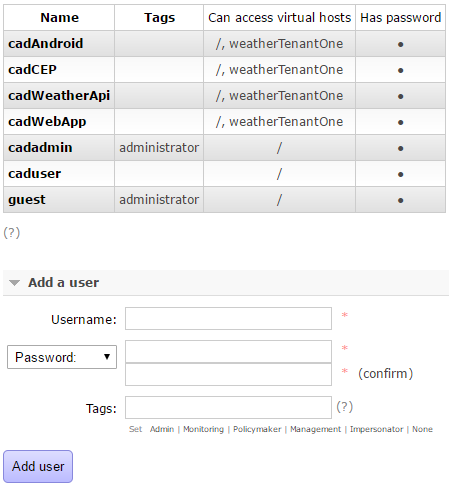
\includegraphics[width=0.5\textwidth]{Bilder/createUser.png}
	\caption{Administrationsmenü zur Benutzererstellung }
	\label{img:AdminCreateUser}
\end{figure}
Die Erstellung neuer Nutzer und die Verwaltung der Rechte erfolgt über unter anderem über das Management Plugin. In Abb. \ref{img:AdminCreateUser} ist ersichtlich, dass die User \textit{cadAndroid}, \textit{cadCEP}, \textit{cadWeatherApi} und \textit{cadWebApp} Zugriff auf den gemeinsamen vHost weatherTenantOne haben. Durch dieses Verfahren kann das gleiche Topic von mehreren Nutzern mit unterschiedlichen vHosts verwendet werden, ohne das sie die Nachrichten anderer vHosts des gleichen Topics lesen können. 
\begin{figure}[htbp]
	\centering
	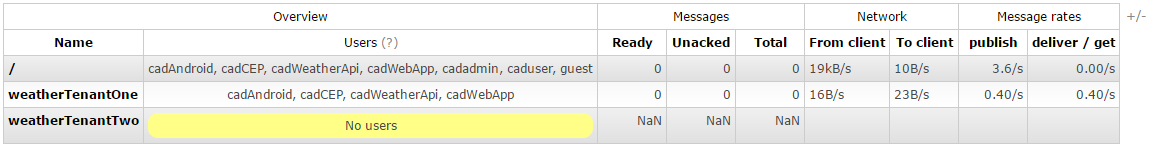
\includegraphics[width=1.0\textwidth]{Bilder/vHostsOverview.png}
	\caption{Übersicht über die virtuellen Hosts}
	\label{img:vHostOverview}
\end{figure}
Eine Übersicht über die einzelnen vHosts und die berechtigten Nutzer wird in Abb. \ref{img:vHostOverview} dargestellt. Diese zeigt noch einmal die erwähnte Zugriffsbeschränkung auf die vier Nutzer dieses Use-Cases sowie den aktuell verursachten Datentransfer der vHosts. Auf diese Weise erfüllt die Anwendung die Anforderung der Multi-Tenancy. Die Persistierung der Nutzerdaten erfolgt in die RabbitMQ-eigene Datenbank. Leider erfolgt die Persistierung in Verbindung mit dem Hostnamen der aktuellen Instanz. Dies führt dazu, dass bei der Änderung des Containers die Task Definition aktualisiert werden muss und dadurch automatisch die Instanz neu gestartet wird, wodurch sich der Hostname ändert und die Datenbank leer gestartet wird. Dieses Problem wird bereits sehr häufig thematisiert. Leider konnte keiner der Lösungsvorschläge das Problem beheben. Da dieser Fall nicht häufig auftritt und der RabbitMQ-Container kein Teil des Continuous Delivery Prozesses ist, wurde durch das Team eine Lösung entwickelt, um die dadurch entstandenen Probleme zu minimieren. Die Umsetzung wird in Absatz \ref{momservice} erläutert. Zusätzlich zum Management Plugin bietet RabbitMQ eine HTTP-Schnittstelle, diese ermöglicht es dem Administrator zum einen über eine Kommandozeile in Verbindung mit Kommandozeilenprogrammen wie cURL (Client for URLs) die angebotenen Schnittstellen aufzurufen und dadurch unter anderem Nutzer anzulegen oder die Verbindungsraten der vHosts auszugeben und auszuwerten (vgl. https://pulse.mozilla.org/api/). Aufgrund der vorhandenen Schnittstellen bietet sich dem Entwickler die Möglichkeit, die Administration über eine eigene Applikation durchzuführen. 
\clearpage
\subsection{12 Faktor App}\label{12FactorApp}
In diesem Absatz wird dargestellt, ob und wie die Anforderungen umgesetzt wurden.
\begin{table}[ht]
  \centering
    \begin{minipage}{17cm}
      \centering
      \begin{tabular}{*{3}{|l|p{3.0cm}|p{7.0cm}}}\hline
      \multicolumn{4}{|c|}{\cellcolor[RGB]{200,200,200}Validierung nach "12 Faktor APP"}\\\hline
     \textbf{ID}&\textbf{Anforderung}&\textbf{Validierungs Element}&\textbf{Erfüllt}\\\hline
     1.&Codebase&Andere Komponenten sind nur für das Testszenario da. Deployment verschiedener Versionen über Repo möglich&Ja\\
      \hline
     2.&Abhängigkeiten&Keine Abhängigkeiten zu anderen Komponenten&Nein\\
     \hline
     3.&Konfiguration&Konfigurationsdatei wird beim Start des Containers aufgerufen und schränkt den Gast-Zugang auf localhost ein. Credentials werden über Umgebungsvariablen im Amazon Container Service (ACS) gepflegt.&Ja\\
     \hline
     4.&Unterstützende Dienste&Keine unterstützenden Dienste vorhanden&Nein\\
     \hline 
     5.&Build, release, run& Könnte durch Jenkins verwaltet werden. Da die MOM keine regelmäßigen Update-Zyklen durchläuft, wurde darauf verzichtet.&Möglich,\- nicht aktiv\\
     \hline
     6.&Prozesse&Der Start des RabbitMQ wird durch das init-Skript im Dockerfile gesteuert. Dieses wird durch dem CMD-Befehl automatisch ausgerufen, so dass der Anwender nur den Task im ACS starten muss (ref{acs}).&Ja\\
     \hline
      7.&Bindung an Ports&Notwendige Ports werden über die EXPOSE-Befehle im Dockerfile deklariert. Das Mapping dieser Ports wird in den Container-Einstellungen von ACS definiert. &Ja\\
     \hline
     
       \hline
      \end{tabular}
    \end{minipage}
    \caption{Validierung der CEP nach "12 Faktor APP (1)"}\label{tab:AnforderungenCEP}
\end{table}

     \begin{table}[ht]
  \centering
    \begin{minipage}{17cm}
      \centering
      \begin{tabular}{*{3}{|l|p{3.0cm}|p{7.0cm}}}\hline
     \textbf{ID}&\textbf{Anforderung}&\textbf{Validierungs Element}&\textbf{Erfüllt}\\\hline 
 8.&Nebenläufigkeit&Die Skalierung kann über ACS erfolgen. ACS ist bereits hoch skalierbar und bietet dem Verwalter des Containers die Konfiguration der Skalierung an. So können Minimum- und Maximum-Tasks sowie eine gewünschte Anzahl an Tasks definiert werden. Die Anzahl der laufenden Tasks bestimmt die Anzahl der laufenden Instanzen. Im verwendeten Nutzungsplan von ACS ist eine Instanz im Mittel über einen Monat verteilt kostenlos verfügbar.&Ja\\     
      \hline
      9.&Einweggebrauch&Der Container kann schnell stoppt und gestartet werden. Durch Probleme mit der RabbitMQ-eigenen Datenbank besteht dann allerdings die Gefahr, im laufenden Betrieb hinzugefügte Nutzer neu hinzufügen zu müssen, da diese bei RabbitMQ auf den Namen des Hosts gespeichert werden und sich dieser beim Neustart des Containers ändert. Ein Workaround wurde entwickelt, dieser aktualisiert aber lediglich das Init-Skript und fügt diesem die Nutzer automatisch hinzu. Dadurch muss beim Neustart auch das Skript aktualisiert werden. &Teilweise\\
     \hline
     10.&Dev-Prod-Vergleichbarkeit&Containerisierung durch Docker (\ref{Docker}).&Ja\\
     \hline     
     11.&Logs&Das Docker-Image von RabbitMQ gibt die Log standardmäßig über Stdout (tty) aus&Ja\\
     \hline
     12.&Admin-Prozesse&Automatische Ausführung eines Skripts beim Containerstart&ja\\
       \hline
      \end{tabular}
    \end{minipage}
    \caption{Validierung der CEP nach "12 Faktor APP (2)"}\label{tab:AnforderungenCEP2}
\end{table}
\section{Wetter-API(Datenquelle)}
In diesem Kapitel wird auf die im Rahmen dieses Projektes Wetter-API vom Anbieter "OpenWeatherMap" eingegangen und anschließend eigens dafür implementierte Services zu dieser beschrieben. Anschließend werden die für den Services implementierten Klassen, Methoden und Tests beschrieben. Abschließend wird diese Komponente gegen die zu Beginn definierten Anforderungen validiert. 
\subsection{Die API}
Der Anbieter "OpenWeatherMap" bietet kostenlos die Möglichkeit Wetterdaten via HTTP-Request abzufragen. 
Hierzu ist lediglich ein Nutzerzugang erforderlich, welchen sich jeder anlegen kann. Es können verschiedene Vorhersagen abgefragt werden, für diese Arbeit beschränkt es sich jedoch auf die tägliche Vorhersage und eine  5-tages Vorhersage. Solch ein angesprochener HTTP-Request (hier für eine 5-tägige Vorhersage) setzt sich wie folgt zusammen, 
\begin{lstlisting}
http://api.openweathermap.org/data/2.5/forecast?zip=78467,de&
APPID=41c464d95d33fabc24d44a5086ea9848
\end{lstlisting}

Der Parameter "ZIP" wird zum setzten der Postleitzahl für die gewünschte Stadt genutzt, zu diesem muss noch das Länderkürzel hinzugefügt werden. Die "APPID" wird von "OpenweatherMap" für jeden Nutzeraccount spezifisch vergeben und dient als Authentifizierung. Der Parameter"forecast" dient zur Unterscheidung zwischen einer aktuellen Vorhersage und einer 5-tages Vorhersage, bei Erster würde der Request wie folgt aussehen, 

\begin{lstlisting}
http://api.openweathermap.org/data/2.5/weather?zip=78467,de&
APPID=41c464d95d33fabc24d44a5086ea9848
\end{lstlisting}

hier muss lediglich der Parameter "forecast" durch "weather" ersetzt werden. 

"OpenWeatherMap" unterscheidet das Angebot zwischen kostenfrei und kostenpflichtig. Innerhalb der kostenpflichtigen Varianten gibt es Staffelungen, das gesamte Angebot wird aus Abb. \ref{img:OpenWeather} genauer ersichtlich. 

Für die in dieser Arbeit beschriebenen Lösung wurde auf die kostenfreie Variante gesetzt. Daher musste bei der Implementierung auf einige Einschränkungen geachtet werden, zu diesen gehören, 
TODO erkläre die Einschränkungen
\begin{itemize}
\item "Calls per minute (no more than)",
\item "Availibilty",
\item "Weather API data update".
\end{itemize}

Da auf das kostenfreie Modell gebaut wird, muss vor allem auf die erstgenannte Einschränkung (Abb. \ref{img:OpenWeather}) geachtet werden. Laut dieser sind lediglich 60 Requests mit den oben gezeigten URLs erlaubt. Im Rahmen der gesamten Anwendung wurde entscheiden, dass diese Applikation für alle Hauptstädte der 16 Bundesländer und Konstanz zur Verfügung stehen soll. Somit errechnet sich der Anteil an Requests pro Minute wie folgt,

\begin{align}
RequestsPerMin. = (16*2)+(2*2)\\
RequestsPerMin. = 36
\end{align}
somit kann ohne auf Probleme zu stoßen, ein Request-Intervall von 60 Sekunden, gewählt werden. 

\begin{figure}[!ht]
	\centering
	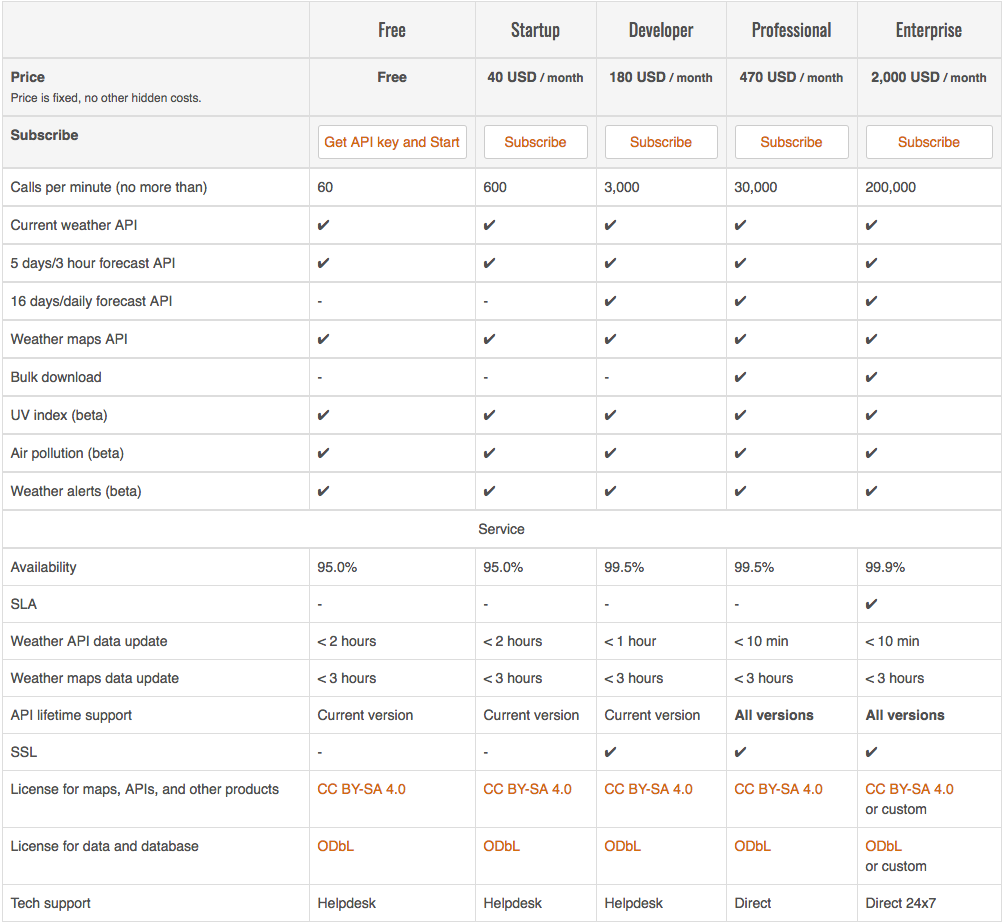
\includegraphics[width=1.0\textwidth]{Bilder/OpenWeatherMap.png}
	\caption{OpenWeatherMap Konditionen}
	\label{img:OpenWeather}
\end{figure} 
Im Bezug auf den "Response-Type" der API, kann entschieden werden, ob als "Response-Type" das JSON- oder XML-Format gewählt werden soll. Aufgrund der guten Möglichkeiten von Java mit JSON-Dokumente zu arbeiten, wurde  das JSON-Format, als "Response-Type", gewählt.
Um bessere Vorstellungen von solch einem Response im JSON-Format zu bekommen wird dieser untenstehend am Beispiel einer täglichen Vorhersage gezeigt.  

  \begin{lstlisting}
{"coord":{"lon":9.16,"lat":47.67},"weather":[{"id":800,"main":"Clear","description":"clear sky","icon":"01d"}],"base":"stations","main":{"temp":297.6,"pressure":1021,"humidity":41,"temp_min":296.15,"temp_max":298.15},"visibility":10000,"wind":{"speed":5.7,"deg":30},"clouds":{"all":0},"dt":1497797400,"sys":{"type":1,"id":4915,"message":0.0038,"country":"DE","sunrise":1497756293,"sunset":1497813872},"id":0,"name":"Konstanz","cod":200}
\end{lstlisting}

Des weiteren wird am nächsten Beispiel der Response-Type für die 5-tägige Vorhersage aufgezeigt, jedoch wird hier aufgrund des hohen Umfangs nur ein kleiner Teil (für 3 Stunden) gezeigt. Im Normalfall besteht ein vollständiger Response aus im 3 stunden Takt 
folgenden Informationen für 5 Tage.
 
  \begin{lstlisting}
{"cod":"200","message":0.0035,"cnt":40,"list":[{"dt":1497808800,"main":{"temp":295.56,"temp_min":294.226,"temp_max":295.56,"pressure":957.98,"sea_level":1034.02,"grnd_level":957.98,"humidity":53,"temp_kf":1.34},"weather":[{"id":800,"main":"Clear","description":"clear sky","icon":"01d"}],"clouds":{"all":0},"wind":{"speed":2.46,"deg":51.5021},"sys":{"pod":"d"},"dt_txt":"2017-06-18 18:00:00"}
\end{lstlisting}
\clearpage
Um mit diesen JSON-Response-Types besser und freier arbeiten zu können wurde ein Service implementiert, welche die Daten vorher Filtert, somit werden nur wichtige Informationen genutzt. Die Implementierung dieses Services wird im folgenden Abschnitt beschrieben. Der Service greift die Grundlagen und Problemstellungen der "OpenWeatherMap"-API auf, welche in diesem Abschnitt beschrieben wurden, von den Request-Intervallen bis hin zu den zwei verschiedenen Arten von Vorhersagen.

\subsection{Die Komponenten und Klassen}

Im untenstehenden Diagramm Abb.\ref{img:KomponentenWetterAPI} werden die einzelnen Teilkomponenten der in diesem Kapitel beschrieben Wetter-API sowie den zur Behebung des erläuterten RabbitMQ-Problems zusätzlich implementierten Komponenten gezeigt.

\begin{figure}[!ht]
	\centering
	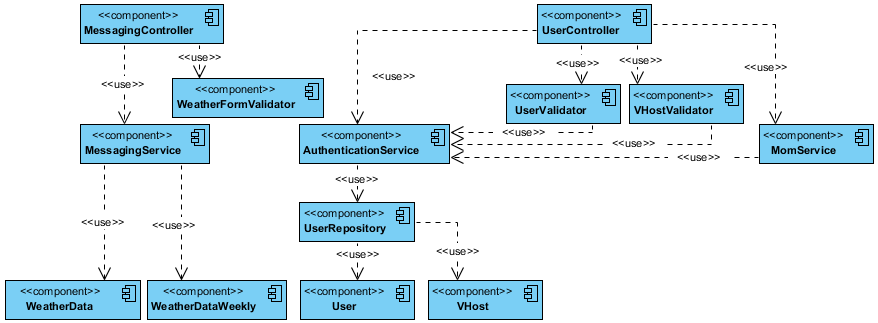
\includegraphics[width=1.0\textwidth]{Bilder/WetterApiKomponentendiagramm.PNG}
	\caption{Wetter-API Komponenten}
	\label{img:KomponentenWetterAPI}
\end{figure} 

Die zugrundeliegenden Klassen der einzelnen Komponenten werden im folgenden kurz beschrieben. Anschließend wird in den nächsten Abschnitten auf die wichtigsten Klassen und die darin enthaltenen Methoden noch genauer eingegangen. 

\begin{description}


\item[MessagingController:]Diese Klasse nimmt die Aufrufe der Wetterformulare der Startseite entgegen und leitet sie an den MessagingService weiter

\item[UserController:]Der User-Controller enthält die REST-Schnittstellen für den Login, die Registrierung neuer Nutzer und die Vergabe von Rechten. 
\item[User:]Die Userklasse beinhaltet die Attribute zur Persistierung und Verwaltung der Nutzerdaten.
\item[VHost:] Die Klasse VHost enthält den Namen des virtuellen Hosts, den Namen des Nutzers dessen Rechte geändert werden sowie die Ausprägung der Rechte, unterteilt in Lese-, Schreib- und Konfigurationsrechte.
\item[WeatherData:]Die Klasse dient als Grundlage für die Datenstruktur der täglichen Daten des JSON-Reponse, welche von der Klasse WeatherAPIService an die MOM gesendet werden. 
\item[WeatherDataWeekly:]Die Klasse dient als Grundlage für die Datenstruktur der wöchentlichen Daten des JSON-Reponse, welche von der Klasse WeatherAPIService an die MOM gesendet werden. 
\item[AuthenticationService:]Diese Klasse dient dem Aufruf der notwendigen Methoden im UserRepository.
\item[UserRepository:]Über das UserRepository erfolgt der Zugriff auf die hinterlegte Datenbank.
\item[WeatherApiService:]Die Klasse vom Typ MessagingService regelt die HTTP-Requests an die "OpenWeatherAPI" und ließt die HTTP-Responses aus, diese Klasse wird im nächsten Abschnitt noch genauer eingeführt, da sie essentiell ist. 

\item[MomService:]Über den MomService erfolgt der Zugriff auf die HTTP-API von RabbitMQ.
\item[SecurityService:]Durch den SecurityService wird der Name des eingeloggten Nutzers ermittelt.

\item[UserDetailsService:]Der UserDetailService ist eine Klasse von Spring Security und lädt einen User und seine Rechte.

\item[UserValidator:]Mit Hilfe des UserValidators erfolgt die Validierung des Registrierungsformulars auf ungültige Passwörter und bereits vorhandene Nutzernamen.
\item[VHostValidator:]Durch den VHostValidator werden die Eingaben im Formular zur Vergabe von Rechten validiert. 
\item[WeatherFormValidator:]Der WeatherFormValidator überprüft, ob alle notwendigen Eingaben zur Erstellung eigener Wetterdaten vorhanden sind.
\item[WeatherApiApplication:]Diese Klasse ist die Startklasse der Spring-Boot Applikation und lädt die properties-Dateien welche die Nachrichten der verschiedenen Validierungsklassen enthalten.
\item[WebSecurityConfig:]In dieser Klasse wird definiert, auf welche URLs dieser Anwendung ohne gültigen Login zugegriffen werden kann.

\end{description}

\subsubsection{Wetter-API-Service}

Für den Zugriff und die Abfrage der "OpenWeatherMap“-API wurde ein Service mit der Klasse "WeatherDataService" implementiert, welcher die Abfrage regelt und ein JSON mit der gewünschten Struktur zurückliefert. Dieses JSON wird dann mit Hilfe von "MQTT" an die MOM (vgl. Kap.\ref{rabbitmq}) gepublished. 

Die gesamte Komponente verfügt über einen Web-Client. Dieser Web-Client stellt die Möglichkeit bereit Testdaten an die MOM zu senden oder aber die Abfrage der Wetterdaten an die "OpenWeatherMap"-API zu starten. Da für die gesamte Applikation die Livedaten von grundlegender Wichtigkeit sind, muss dieser Service zu jeder Zeit laufen. Es ist im Realbetrieb nicht vorgesehen, dass dieser gestoppt wird.

Nachfolgend werden die wichtigsten Methoden der Klasse "WeatherDataService" beschrieben. 

\begin{description}
\item["init()"] füllt eine HashMap mit allen gewünschten Postleitzahlen auf, nach welchen die "OpenWeatherMap"-API abgefragt werden soll.
\item["public void publishLiveWeatherData()"] ruft im Intervall von 60 Sekunden die Methoden "handlePLZtoday(plz, countryCode)“ und „handlePLZweekly(plz, countryCode)“ mit allen Postleitzahlen und Countrycodes auf, welche in der Init() -Methode eingelesen wurden. 
\item["public void handlePLZtoday(String plz, String countryCode)"] stellt einen HTTP-Request und fragt die tagesaktuellen Wetterdaten im JSON-Format ab.
\item["public void dailyToWeatherData(...)"] liest den von der Methode "handlePLZtoday" gestellten HTTP-Request aus und zieht die gewünschten Daten anhand der Struktur der Klasse "WeatherData" aus dem Response-JSON der "OpenWeatherMap"-API. Anschließend wird  die gewünschte JSON-Struktur zusammengebaut. 
\item["public void handlePLZweekly(String plz, String countryCode)"]stellt einen HTTP-Request und fragt die 5-tägigen Wetterdaten im JSON-Format ab.
\item["public static ArrayList WeatherDataWeekly weeklyToWeatherDataWeekly 
(...)" ]liest den von der Methode "handlePLZweekly" gestellten HTTP-Request aus und zieht die gewünschten Daten anhand der Struktur der Klasse "WeatherDataWeekly" aus dem Response-JSON der "OpenWeatherMap"-API. Anschließend wird die gewünschte JSON-Struktur zusammengebaut.
\item["private void reconnectToMoM()"] stellt sicher, dass bei einem Verbindungsverlust zur MOM wieder eine Verbindung hergestellt wird. 
\item["public void publishFakeWeatherData(WeatherData weatherData)"] sendet die Daten, via Web-Client eingepflegt wurden, an die MOM. 
\end{description}

Im nachfolgenden Abschnitt wird die Implementierung zur Lösung des in Absatz \ref{rabbitmq} erläuterten Problems beschrieben. Dafür wurde ein Registrierungs- und Rechtevergabeprozess implementiert. Auf Grundlage der dabei erstellten Datensätze wird zum Abschluss eines Registrierungsprozesses oder der Vergabe von Rechten das init.sh Shellskript erstellt. Dieses kann dem Dockerimage hinzugefügt werden und legt beim Start eines Containers automatisch die Nutzer in RabbitMQ an.
Damit der Zugriff auf die Registrierungs- und Rechteseite auf den Administrator beschränkt ist, wird dies in der Klasse WebSecurityConfig so definiert. In der selben Klasse werden auch die REST-Schnittstellen definiert die ohne Authentifizierung erreichbar sind. Ruft der Nutzer eine Schnittstelle auf, für die eine Authentifizierung oder eine andere Rolle notwendig ist, erscheint ein Login-Fenster. Die REST-Schnittstellen für den Login und die Rechtevergabe der virtuellen Hosts erfolgt über den UserController. Im UserController erfolgt die Persistierung und Validierung der Daten mit der in Kapitel 5 erläuterten Datenbank durch den Authentifizierungsservice. Gleichzeitig werden die Daten dieser Nutzer über die HTTP-API von RabbitMQ in selbigem gespeichert. Dies erfolgt durch den MomService.
\subsubsection{Authentifizierungsservice}\label{momservice}
Der Authentifizierungsservice wird über den UserController aufgerufen. Der Service selbst wird für den Login-Prozess, die Registrierung neuer Nutzer und die Rechtevergabe für die virtuellen Hosts aufgerufen. Der Login-Prozess wird dabei vollständig von Spring Security übernommen. Wird ein neuer Nutzer registriert, erfolgt zuerst die Validierung der eingebenen Daten durch den UserValidator. Dabei wird geprüft, ob der Nutzer bereits vorhanden ist und das Passwort mit dem Bestätigungspasswort übereinstimmt. Bei einer fehlerhaften Eingabe oder einem bereits vorhandenen Nutzer wird die entsprechende Ausgabe auf der Weboberfläche ausgegeben. War die Validierung erfolgreich, wird die Methode createUser(userForm) aufgerufen. Diese ruft die Methode insertSystemUser(Username, encodedPassword, Description) auf. Die Verschlüsselung des Passworts erfolgt über den BCryptPasswordEncoder von Spring Security. Im UserReposity werden die notwendigen SQL Statements aufgerufen, um den Nutzer in der Datenbank zu sichern. Die Vergabe von Rechten für virtuelle Hosts erfolgt über die Methode addPermission(vHostForm) des Authentifizierungsservices. Die vHostForm wird vorab durch den VHostValidator geprüft, ob der zugewiesene Nutzer bereits existiert. Anschließend erfolgt der Aufruf der addPermission-Methode und die Speicherung der Rechte des Nutzers für den virtuellen Host in der Datenbank über das UserRepository.
\subsubsection{MOM-Service}
Neben den Speicherung der Nutzer und Berechtigungen in der Datenbank müssen diese ebenfalls im RabbitMQ gespeichert werden. Dies erfolgt im MOM-Service. Der Service enthält dazu die Methoden addUser(loggedInUser, userToSave), setPermission(loggedInUser, userToSave, vHost) und createVHost(loggedInUser, vHost). Diese Methoden greifen über definierte Schnittstellen der HTTP-API auf RabbitMQ zu. Die Variable loggedInUser wird benötigt, um mit dessen Zugangsdaten über einen curl-Request die notwendigen Schnittstellen aufzurufen. Dies ist nur möglich, wenn der eingeloggte Nutzer Administrator-Rechte auf der RabbitMQ-Instanz hat. Zusätzlich enthält der MOM-Service die Methode writeScript(). Durch diese Methode werden die aktuellen Nutzer und ihre Rechte aus der Datenbank geladen und als rabbitmqctl-Aufruf im init-Skript für das Containerimage gespeichert. Das Skript kann in ein Repository für das Containerimage gespeichert werden. Beim der Ausführung des Dockerfiles  wird das Skript als Startpunkt für den Container definiert. Wird der Container gestartet, erfolgt die Ausführung des Skripts und die Nutzer werden gemeinsam mit den aus der Datenbank ermittelten Berechtigungen beim Start des Containers angelegt. Auf das Deployment des Dockercontainers wird in Absatz \ref{Docker} noch genauer eingegangen.




%\subsection{Testing}
%Im Rahmen des Testings wurde für die Klasse "WeatherAPIService" eine Testklasse "WeatherAPIServiceTest" angelegt. 
%Diese Klasse testet die wichtigsten Methoden der Ursprungsklasse, zu den Testmethoden gehören,

%\begin{itemize}
%\item "testAPICallTodayWithoutWindDeg()"
%\item "testAPICallTodayWithWindDeg()"
%\item "testAPICallWeeklyWithoutWindDeg()"
%\item "testAPICallWeeklyWithWindDeg()"
%\end{itemize}

%Die ersten zwei Methoden Testen, für den Fall eines HTTP-Response seitens der API für eine tagesaktuelle Wettervorhersage. Dafür wurde ein String mit gefakten Daten angelegt, mit diesen Daten wurde dann die Methode "dailyToWeatherData" aufgerufen, somit kann sichergestellt werde, dass die endgültige Form des JSON mit der gewünschte der "WeatherData" Klasse übereinstimmt. 
%Hier muss jedoch eine Fallunterscheidung gemacht werden, da in der Methode noch mit Hilfe einer Kontrollstruktur der Fall %angefangen wird, dass die API für die Windrichtung keinen Wert sendet. Dieser Fall tritt immer dann ein, wenn die Windstärke unter den Wert 1.5 sinkt. Aus diesem Grund gibt es, wie oben angegeben, diese zwei Fallunterscheidung bei den Testmethoden. 

%Die weiteren zwei Methoden testen einen fast anlogen Fall zu den ersten zwei ab nur das hier ein HTTP-Response für eine 5-tägige Wettervorhersage getestet wird. Der unterschied besteht in der Konstruktion der Testdaten, da diese eine komplexere und größere Menge aufweisen, als in den ersten beiden Fällen. Aus dem Grund wurden 2 Hilfsmethoden implementiert, welche einen String bauen, welcher gleich einem API-Response für eine 5-tägige Vorhersage ist.

\subsection{12 Faktor App}\label{12FactorAppWeatherAPI}

\begin{table}[!ht]
  \centering
    \begin{minipage}{15cm}
      \centering
      \begin{tabular}{*{3}{|l|p{5.0cm}|p{5.0cm}}}\hline
      \multicolumn{4}{|c|}{\cellcolor[RGB]{200,200,200}Validierung nach "12 Faktor APP"} \\\hline
     \textbf{ID}&\textbf{Anforderung}&\textbf{Validierungs Element}&\textbf{Erfüllt}\\\hline
     1.&Codebase&Andere Komponenten sind nur für das Testszenario da. Deployment verschiedener Versionen über Repo möglich&Ja\\
      \hline
     2.&Abhängigkeiten&Zugriff auf die Datenbank und die "OpenWeatherMap"-API sind in eigenen Klassen isoliert&Ja\\
     \hline
     3.&Konfiguration&Credentials werden über Umgebungsvariablen im Jenkings-Server verwaltet&Ja\\
     \hline
     4.&Unterstützende Dienste&Credentials der "OpenWeatherMap"-API werden über die Umgebungsvariablen im Jenkins-Server verwaltet&Ja\\
     \hline 
     5.&Build, release, run&Wird über einen Jenkins-Server verwaltet&Ja\\
     \hline
     6.&Prozesse&Wird via Web-Gui gestartet&Ja\\
     \hline
      7.&Bindung an Ports&Die Ports werden von Pivotal verwaltet&Ja\\
     \hline
     8.&Nebenläufigkeit&Es könnte zu jeder Zeit eine neue Instanz auf Pivotal gestartet werden, jedoch bedarf es bei dieser Komponente keiner Skalierung&Ja\\
     \hline
      \end{tabular}
   \caption{Validierung nach "12 Faktor APP"}\label{tab:Anforderungen}
    \end{minipage}
\end{table}

\begin{table}[!h]
  \centering
    \begin{minipage}{15cm}
      \centering
      \begin{tabular}{*{3}{|l|p{5.0cm}|p{5.0cm}}}\hline
      \multicolumn{4}{|c|}{\cellcolor[RGB]{200,200,200}Validierung nach "12 Faktor APP"} \\\hline
     \textbf{ID}&\textbf{Anforderung}&\textbf{Validierungs Element}&\textbf{Erfüllt}\\\hline

      9.&Einweggebrauch&Pivotal generiert aus der hochgeladenen .jar oder .war einen Container, welcher jeder Zeit über die GUI in Pivotal gestoppt werden kann. &Ja\\
     \hline
     10.&Dev-Prod-Vergleichbarkeit&Containerisierung durch Pivotal&Ja\\
     \hline     
     11.&Logs&Pivotal gibt die Logs standardmäßig über Stdout aus&Ja\\
     \hline
     12.&Admin-Prozesse&Nicht vorhanden&Nein\\
     \hline
      \end{tabular}
   \caption{Validierung nach "12 Faktor APP"}\label{tab:Anforderungen}
    \end{minipage}
\end{table}
\section{Datenverarbeitung}\label{db}

Eine gehostete Datenbank eröffnet unserem WetterAPI-System viele weitere Möglichkeiten. Neben System User Informationen der Messaging-Oriented Middleware RabbitMQ ,  können die empfangenen Wetterdaten kontinuierlich abgespeichert werden. Die hinterlegten Daten können nun für eine Reihe von Statistiken und Auswertungen genutzt werden und bieten außerdem den Vorteil  den künftigen Ressourceneinsatz und die Skalierung effizienter zu gestalten. 
In diesem Kapitel wird der Aufbau einer passenden Datenbank  beschrieben. Da das Testen eines skalierbaren Datenbankservices in der Regel sehr teuer ist, werden einige Funktionalitäten nur in der Theorie beschrieben. Dennoch lässt sich der Nutzen eines Datenbankkonzepts klar herausstellen.
Zur Speicherung der Datensätze wird ein relationales Datenbankschema auf MYSQL Basis verwendet. Gehostet wird über den Amazon Web Service Dienst RDS. Für eine einfache Implementierung und Verwendung der Datenbank in den Systemmodulen CEP und MQTT (RabbitMQ) wird eine JDBC Schnittstelle zur Verfügung gestellt.

\subsection{Datenbankschema}

\textbf{System User und VHost ER Modell}
Das Datenbankschema lässt sich in 2 verschiedene Bereiche unterteilen. Neben einer Speicherstruktur für die eingehenden Wetterdaten, lassen sich auch User Accountinformationen der RabbitMQ abspeichern. In Abbildung \ref{img:DBSchemaSystemUser} ist das Schema der Tabellenkonstellationen für die Speicherung der SystemUser zu sehen: 
\begin{figure}[htbp]
	\centering
	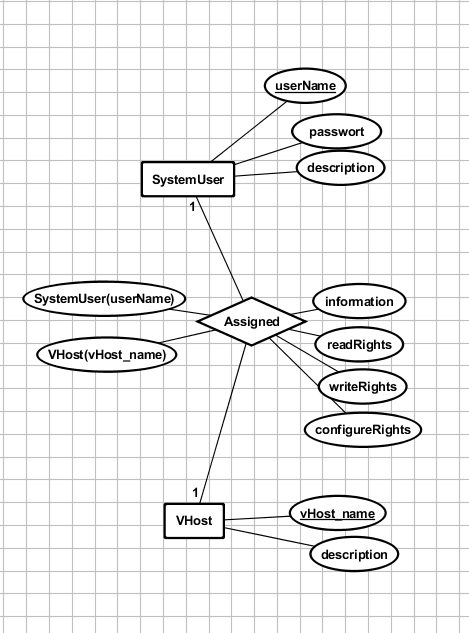
\includegraphics[width=0.5\textwidth]{Bilder/DBSchemaSystemUser.png}
	\caption{Datenbank ER Modellierung - Rabbit MQ System Data}
	\label{img:DBSchemaSystemUser}
\end{figure} 
Die Tabelle SystemUser  beinhaltet die LogIn Credentials und die Tabelle VHost lässt die Sicherung der RabbitMQ Informationen zu. 
Die n:m Beziehung zwischen System Usern und VHost wird in der Tabelle Assigned abgebildet. Hier lassen sich auch die jeweiligen Berechtigungen read, write und configure des Users auf der RabbitMQ Instanz hinterlegen.

\textbf{Wetter Daten ER Modell}
Damit die eingehenden Daten der WetterAPI  korrekt abgelegt werden können, sind Stammdaten in der Datenbank gepflegt. Neben den zur Verfügung stehenden Städten in der Tabelle City, werden auch die Standardwetterdaten (Tabelle DeaultWeather) aus der verwendeten WetterAPI hinterlegt. Jedes eingehende  Wetterdatenobjekt ist einer Stadt zugeordnet und referenziert ein DefaultWeather Eintrag.
Die User unserer Systemlösung können ebenfalls in der Datenbank gespeichert werden. Die Tabelle Subscribe beinhaltet die n:m Referenzen von Usern, welche bestimmte Städte beziehungsweise deren Wetterdaten abonniert haben. Jeder Eintrag in der Tabelle Subscribe besitzt zudem das Datum der Aktivierung des Abonnements. Abbildung \ref{img:DBSchemaWetterDaten} visualisiert das ER Modell der Wetterdatenspeicherung:
\begin{figure}[htbp]
	\centering
	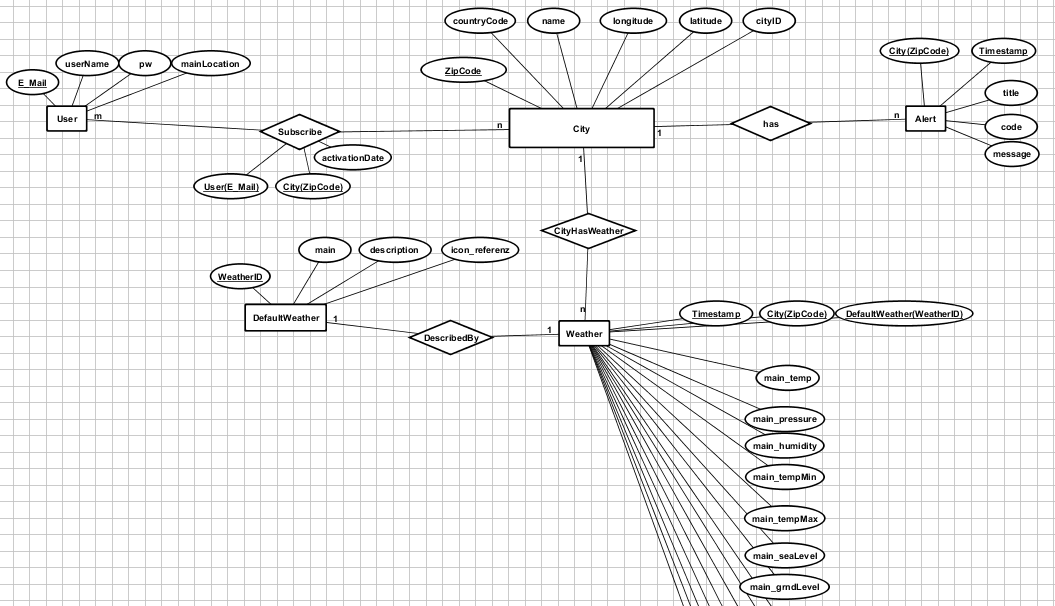
\includegraphics[width=0.5\textwidth]{Bilder/DBWetterDaten.png}
	\caption{Datenbank ER Modellierung - Wetter Daten Modellierung}
	\label{img:DBSchemaWetterDaten}
\end{figure} 
Die Central Processing Unit, kurz CEP, errechnet anhand der eingehenden Wetterdaten verschiedene Benachrichtigungen (Alerts), welche über die MoM als Topic an die User verteilt werden. In der Datenbank können diese Alerts in Abhängigkeit der betroffenen Stadt gespeichert werden.

\subsection{Datenbank – JDBC Schnittstelle}
Der Zugriff und die Verwaltung der Datensätze nach dem, im vorherigen Kapitel beschrieben, Datenschema, ist in der Java Klasse  CadWeatherSystemDatabaseAPI realisiert. Diese Klasse lässt sich in alle Teilmodule unseres Gesamtsystems implementieren und bietet eine Schnittstellefunktionalität zur Verwendung der Datenbankinstanzen. In den Java Methoden, werden die MYSQL Kommunikationssatetments codiert als String über ein connection Objekt auf der Datenbank ausgeführt. Grundsätzlich stehen INSERT Operationen für alle Tabellen, sowie diverse SELECT Abfragemöglichkeiten zur Verfügung. Ziel dieser Struktur ist eine simple, vereinheitlichte Methodik zur Benutzung der Datenbankinstanzen.
Der Konstruktor der Klasse gibt dem Entwickler die Möglichkeit ein MYSQL Datenbankobjekt in die Schnittstelle einzubinden.

In der nachfolgenden Tabelle sind alle derzeit programierten Methoden aufgelistet.
Die INSERT  Methoden liefern das Feedback der Datenbankoperation in einem String zurück. Die Rückgabe ResultSet der select-Methoden beinhaltet die gefunden Datentupel der Abfrage.

{\bf GENERAL DB}
\begin{itemize}
\item String  checkDatabaseConnection()
\item java.sql.Connection getConnection()
\item setConnection(java.sql.Connection  databaseConnection)
\end{itemize}

{\bf CEP DB - INSERT}
\begin{itemize}
\item String insertDefaultWeather(int WeatherID, String main, String description, String iconReferenz)
\item String insertCity(int ZipCode, String cityName, Double logitude, Double latitude, int cityID)
\item String insertUser(String EMail, String userName, String passwort, int mainLocation)
\item String insertSubcribe(String EMail, int ZipCode)
\item String insertAlert(int ZipCode, Timestamp timestamp, String title, String code, String message)
\item String insertWeather(Timestamp TimeStamp, int ZipCode, int WeatherID, 
				double mainTemp, double mainPressure, double mainHumidity, double mainTempMin,
				double mainTempMax, double mainSeaLevel, double mainGrndLevel,
				String windDirection, double windSpeed, double windDeg, String cloudsDesc, double rain3h, 
				double snow3h, 
				Timestamp sysSunset, Timestamp sysSunrise)
\end{itemize}

{\bf CEP DB - SELECT }
\begin{itemize}
\item ResultSet selectUserByMail(String userEMail)
\item ResultSet selectCityByZipCode(int cityZipCode)
\item ResultSet selectDefaultWeatherByID(int defaultWeatherID)
\item ResultSet selectAllWeatherByCityZipCode(int cityZipCode)
\item ResultSet selectWeatherByCityAndDay(int cityZipCode, Timestamp weatherDay)
\item ResultSet selectWeatherByCityAndTimePeriod(int cityZipCode, Timestamp fromDate, Timestamp toDate) 
\item ResultSet selectSubscribeByUser(String userEMail)
\item ResultSet selectSubscribeByCity(int ZipCode)
\item ResultSet selectUserPwByEMail(String EMail)
\end{itemize}

{\bf Rabbit MQ DB - Insert }
\begin{itemize}
\item String insertSystemUser(String userName, String password, String additionalDescription)
\item String insertVHost(String vHostName, String additionalDescription)
\item String insertAssigned(String systemUserUserName,String vHostName, String additionalInformation, boolean readRights, boolean writeRights, boolean configureRights);
\end{itemize}

{\bf Rabbit MQ DB - SELECT }
\begin{itemize}
\item ResultSet selectVHostAll()
\item ResultSet selectSystemUserAll()
\item ResultSet selectSystemUserByUserName(String userName)
\item ResultSet ResultSet selectAssignedAll()
\end{itemize}



\subsection{Auswertungen und Nutzen der Databankspeicherung}
Die Datensätze können vielseitig genutzt werden. Zum einen hält die CEP Komponente unseres Systems die empfangen Wetterdaten der MoM bzw. der WetterAPI nur temporär. Gleiches gilt für erzeugte Benachrichtigungen in Form von Alerts.
Durch eine Sicherung in der Datenbank stehen die Wetterdaten unabhängig vom Status der CEP persistent zur Verfügung. 
Des Weiteren können verschiedene Auswertungen der Datensätze weitere Erkenntnisse bringen. 

\textbf{Wetter API User}
Durch die Protokollierung der Alerts lassen sich Statistiken über die Ereignisse und deren Verteilung aufstellen. Daraus könnten wir für die User beispielsweise Vorabwarnungen zukommen lassen. Außerdem könnte man den Usern auf lange Sicht gesehen Wettervergleiche bzw. Wetterentwicklungen bereitstellen.

\textbf{Cloud System Analyse}
Mithilfe des gespeicherten Datums der Aktivierung  von User Abonnements zu den jeweiligen Städten, lässt sich auch eine Prognose für unser System erstellen. Je nach Modell der Verteilung der gehosteten Komponenten unseres Systems  können wir aus den Datensätzen abschätzen, wie sich die Last auf unserem System entwickelt. 
Diese Prognosen können für eine Kostenabschätzung des Cloudsytsem wertvoll sein, um Ressourcen effizient einzusetzen und damit verbundene Kostenpunkte besser vorherzusagen.
Selbstverständlich ist der größte Vorteil einer Cloudlösung das dynamische Reagieren auf verschiedene Lastverhalten. Dennoch ist es im Rahmen von Businessmodellen notwendig zu wissen, welche Kosten an welcher Stelle entstehen beziehungsweise geplant werden können.

\subsection{AWS RDS Datenbankverfügbarkeit}
In Bezug auf die Performance spielt bei der Datenbank nur die Anzahl der CEP Calls eine Rolle. Dies führt je nach Szenario und Wetterveränderungen unterschiedlich viele I/O Operationen aus. Dennoch würde unser WetterAPI System selbst bei extrem hohen Userzahlen keine Datenlast liefern, welche die Datenbank an ihre Grenze bringen könnte. Das Bottleneck unseres Systems sind die Instanzen der CEP. Im Rahmen unseres Projektes ist die Skalierung des Datenbank Services nicht eingerichtet, da zusätzliche oder skalierte Datenbankinstanzen mit hohen Kosten verbunden sind, da die benötigten Konfigurationen nicht im Umfang des AWS Trialkontingents enthalten sind. Ganz wichtig ist die Tatsache, dass das Starten einer weiteren Instanz das kostenlose Kontigent an Ressourcen aufhebt. Aus eigener Erfahrung wissen wir, wie sich ein solches Szenario zu einer gewissen Kostenfalle entwickeln kann.
An dieser Stelle sollen dennoch die Möglichkeiten der Datenbankverfügbarkeit in Bezug auf den AWS RDS Dienst beschrieben werden.

\textbf{Vertikale Skalierung}
Die Datenbank empfängt viele write-Operationen, weshalb eine vertikale Skalierung in unserem Fall der beste Ansatz wäre. Amazon bietet in seinem Service RDS (Relationale Datenbank Services) automatische Skalierungsoptionen an. So lassen sich verschiedene Monitoring Parameter (z.B. CPU Auslastung) einstellen, welche beim Erreichen eines Grenzwertes automatisch weitere Kapazitäten zur Verfügung stellt. Der Datenbankinstanz können je nach genutzer Datenbankengine bis zu 32 vCPU's mit 244GB RAM uns bis zu 64TB Datenspeicher zugeschaltet werden. Ein minimaler Nachteil ist eine kurze Downtime Phase in der die neuen Ressourcen eingebunden werden. Es gehen aber keine gespeicherten Daten verloren, sodass man in die Write Operationen der CEP im internen Speicher der CEP halten und bei erneuter Datenbankverfügbarkeit an den RDS Dienst übergeben könnte.

\textbf{Horizontale Skalierung}
Eine horizontale Skalierung eignet sich vor allem bei Applikationen mit einem hohen Anteil an read-Operationen. Hierfür kann man beispielsweise den Amazon Container Service verwenden. Auch hier kann man Amazon konfigurieren, bei einem gewissen Lastverhalten, über einen Dockercontainer eine weitere Instanz aufzuziehen.
Eine weitere Möglichkeit für eine horizontale Skalierung, sind Replica Objekte. Ein Replica Objekt bildet den Aufbau und den Inhalt einer Datenbankinstanz ab und steht für weitere Instanzdeployments zur Verfügung. 

\textbf{Ausfallsicherheit}
Für die Ausfallsicherheit bietet der AWS RDS Dienst die Option Multi-AvailabilityZone. Wenn die Option aktiviert wird, erstellt Amazon eine synchronisierte Datenbankinstanz in einer anderen Region bzw. in einem anderen Rechenzentrum. Beim Ausfall der aktiven Datenbankinstanz wird innerhalb einer Minute die synchrone Datenbankinstanz zugeschaltet und das DNS angepasst, damit sich aus Applikationssicht nichts verändert.


\subsection{12 Faktor App}\label{12FactorApp}
In diesem Absatz wird dargestellt, ob und wie die Anforderungen umgesetzt wurden.


\begin{table}[!ht]
  \centering
    \begin{minipage}{17cm}
      \centering
      \begin{tabular}{*{3}{|l|p{3.0cm}|p{7.0cm}}}\hline
      \multicolumn{4}{|c|}{\cellcolor[RGB]{200,200,200}Validierung nach "12 Faktor APP"} \\\hline
     \textbf{ID}&\textbf{Anforderung}&\textbf{Validierungs Element}&\textbf{Erfüllt}\\\hline
     1.&Codebase&Andere Komponenten sind nur für das Testszenario da. Deployment verschiederner Versionen über Repo möglich&Ja\\
      \hline
     2.&Abhängigkeiten&Keine Abhängigkeiten zu anderen Komponenten&Nein\\
     \hline
     3.&Konfiguration&Konfigurationsdatei wird beim Start des Containers aufgerufen und schränkt den Gast-Zugang auf localhost ein. Credentials werden über Umgebungsvariablen im Amazon Container Service (ACS) gepflegt.&Ja\\
     \hline
     4.&Unterstützende Dienste&Keine unterstützenden Dienste vorhanden&Nein\\
     \hline 
     5.&Build, release, run& Könnte durch Jenkins verwaltet werden. Da die MOM keine regelmäßigen Update-Zyklen durchläuft, wurde darauf verzichtet.&Möglich,\- nicht aktiv\\
     \hline
     6.&Prozesse&Der Start des RabbitMQ wird durch das init-Skript im Dockerfile gesteuert. Dieses wird durch dem CMD-Befehl automatisch ausgerufen, so dass der Anwender nur den Task im ACS starten muss (ref{acs}).&Ja\\
     \hline
      7.&Bindung an Ports&Notwendige Ports werden über die EXPOSE-Befehle im Dockerfile deklariert. Das Mapping dieser Ports wird in den Container-Einstellungen von ACS definiert. &Ja\\
     \hline
      8.&Nebenläufigkeit&Die Skalierung kann über ACS erfolgen. ACS ist bereits hoch skalierbar und bietet dem Verwalter des Containers die Konfiguration der Skalierung an. So können Minimum- und Maximum-Tasks sowie eine gewünschte Anzahl an Tasks definiert werden. Die Anzahl der laufenden Tasks bestimmt die Anzahl der laufenden Instanzen. Im verwendeten Nutzungsplan von ACS ist eine Instanz im Mittel über einen Monat verteilt kostenlos verfügbar.&Ja\\
     \hline
      9.&Einweggebrauch&Der Container kann schnell stoppt und gestartet werden. Durch Probleme mit der Rabbitmq-eigenen Datenbank besteht dann allerdings die Gefahr, im laufenden Betrieb hinzugefügte Nutzer neu hinzufügen zu müssen, da diese bei Rabbitmq auf den Namen des Hosts gespeichert werden und sich dieser beim Neustart des Containers ändert. Ein Workaround wurde entwickelt, dieser aktualiert aber lediglich das Init-Skript und fügt diesem die Nutzer automatisch hinzu. Dadurch muss beim Neustart auch das Skript aktualisiert werden. &Teilweise\\
     \hline
     10.&Dev-Prod-Vergleichbarkeit&Containerisierung durch Docker (\ref{Docker}).&Ja\\
     \hline     
     11.&Logs&Das Docker-Image von Rabbitmq gibt die Log standardmäßig über Stdout (tty) aus&Ja\\
     \hline
     12.&Admin-Prozesse&Automatische Ausführung eines Skripts beim Containerstart&ja\\
     \hline
      \end{tabular}
   \caption{Validierung der CEP nach "12 Faktor APP"}\label{tab:AnforderungenCEP}
    \end{minipage}
\end{table}


\end{document}
\section{Complex Event Process}\label{cep}


\subsection{Zielsetzung}
Das Ziel der Anwendung ist es, die Daten welche an die MoM gesendet wurden auszulesen und dann weiterzuverabeiten. Dabei wird mithilfe einer Complex Event Process Engine dann nach besonderen Ereignissen gesucht. Sollte ein solches eintreffen wird eine Warnung an alle Clients über ein besonderes Topic gesendet. Die Anwendung soll sich dabei ein die 12 Faktoren einer Cloud Anwendung halten. Ein weiteres Ziel ist, dass die Anwendung in jeder Cloud laufen kann und nicht abhängig von einer bestimmten Cloud ist. 

\subsection{Umsetzungsentscheidungen}
Als Complex Process Engine wurde Esper ausgewählt. Da Esper eine Java API besitzt und die MOM ebenenfalls über eine Javaschnittstelle verfügt (Siehe Kapitel \ref{rabbitmq}) kann Esper leicht mit den anderen Komponenten der Anwendung verbunden werden. Esper besitzt zudem eine ausführliche Dokumentation, was die Umsetzung deutlich erleichtert hat. Es gibt neben Esper andere Engines welche ebenfalls mit Java verbunden werden können. Eine davon ist Apache Spark. Spark wird von Amazon direkt unterstüzt und ist eine eigene Engine welche nur noch mit Statements befüllt werden muss angeboten. Wir haben uns aber gegen Spark entschieden, da es zum einen uns stärker an die Amazon Cloud binden würde und zum anderen die Amazon Spark Engine sehr viel abnimmt und so Kontrolle über das Verhalten der Anwendung nimmt. 
\\
Die Anwendung wurde mit Java geschrieben, da es mit Java leicht ist die verschiedenen Komponenten der Anwendung zu verbinden. Java kann überall laufen, sofern eine JVM vorhanden ist. Dadurch haben wir sichergestellt, dass die Anwendung auf jeder Cloud laufen kann. Zusätzlich ist Java die Programmiersprache in der unsere Gruppe die meiste Erfahrung besitzt.   

\subsection{Esper}
Esper ist eine CEP Engine welche von EsperTech entwickelt wurde. Esper ist eine open source Anwendung. Eine Kommerzielle Lizenz wird nur benötigt, wenn die Anwendung weiterverkauft werden soll. Esper arbeitet mit Statements, Listener und Consumption Modes. Esper speichert die eingehenden Events in einer eigenen Datenbank ab und löscht diese von selbst wenn sie nicht mehr benötigt werden. Espers Datenbank wird beim abschalten der Anwendung gelöscht. Esper ist in der Lage verschiedene unabhängige Engines gleichzeitig Laufen zu lassen. 
\\ 
Die Statements basieren auf SQL. Es ist möglich Statements mit Listener zu verknüpfen. Zusätzlich wird der Consumption Mode über die Statements angegeben. Statements können auch verwendet werden um einen Kontext anzugeben. Das wird aber in dieser Anwendung nicht benötigt, daher wird darauf nicht näher eingegangen. In einen Statement wird immer angegeben was genau gesucht wird, woher es kommen soll und was für Filterbedingungen vorhanden sind. Dabei kann in der from-Klausel auch ein Muster stehen. So kann Esper für die Mustererkennung verwendet werden. Die Statements werden auf jedes Event im Eventstrom angewendet. Sollte ein Statement zutreffen wird der dazugehörige Listener aufgerufen. Dieser kann auf die ausgewählten Werte zugreifen. Der Listner kann selbst eigene Events absenden. Der Consumption Mode legt fest ob ein weiterer Listener auf das Event zugreifen kann. Es kann auch festgelegt werden ob ein Längen oder Zeitfenster die Zahl der zuberücksichtigen Events einschränlen soll.   

\subsection{Umsetzung}
Die Anwendung wird von der InformationLifeFlow Klasse gesteuert. Diese stellt die Main-klasse der Anwendung dar und ließt beim Start die Postlleitzahlen der Städte aus. Danach wird eine Verbindung zu einer MoM erstellt. Für jede Postleitzahl wird ein sogennanter MoMReader erstellt. Diese sind eigene Thread welche für ein bestimmtes Topic auf eingehende Nachrichten warted. Der MoMSender ist das Gegenstück dazu. Der Sender sendet Nachrichten zurück zur MoM damit diese von Clients gelesen werden können. Das Klassendiagramm zeigt die Methoden von der Mainklasse und dem Reader.
\begin{figure}[htbp]
	\centering
	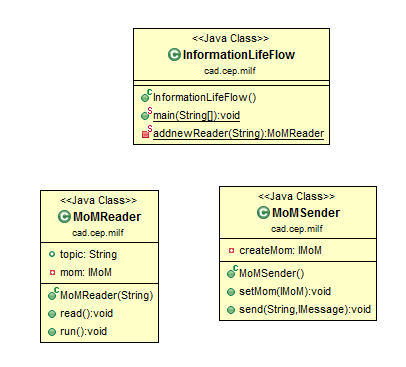
\includegraphics[width=0.5\textwidth]{Bilder/FlowAndReader.png}
	\caption{Klassendiagramm der Steuerungsklassen}
	\label{img:flowDiagramm}
\end{figure} 
Die MoM wird mithilfe einer Factory Klasse erstellt. Diese erstellt beim ersten Aufruf eine MoM und gibt diese bei jeden Aufruf wieder zurück. Derzeit unterstüzt die Anwendung nur eine MQTTMoM. Mithilfe des IMoM interfaces kann aber jederzeit eine weitere MoM hinzugefügt werden. Die MQTT MoM benötigt einen Hostpfad, einen Usernamen und ein Passwort, Diese werden von der Factory aus den Umgebungsvariablen ausgelesen und dann der MoM weitergegeben. Die MoM öffenet eine Verbindung ist dannach in der Lage Nachrichten zu senden oder zu Empfangen. Jede Empfangene Nachricht wird von einer CallBack-Methode ausgewertet. Diese überprüft was für ein Typ die Nachricht besitzt und behandelt diese dann entsprechenend. Das bedeutet ein Forcast wird umgeformt und weitergeleitet während einer Tagesmeldung weiter an die CEP Engine gesendet wird. Beim Umformen des Forcasts wird auch die maximale Temperatur, die minimale Temperatur und das durchschnittswetter für jeden Tag ermittelt. Das folgende Klassendiagramm zeigt die Komponenten der MoMverbindung.
\begin{figure}[htbp]
	\centering
	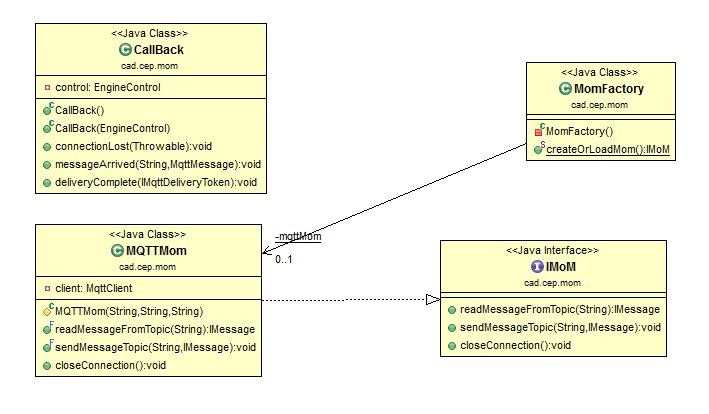
\includegraphics[width=0.5\textwidth]{Bilder/MoMKomponents.png}
	\caption{Klassendiagramm der MoM Komponenten}
	\label{img:MoMDiagramm}
\end{figure} 
Die Anwendung kennt verschiedene Nachrichtentypen. Die Nachrichten die eingehen sind entweder eine Nachricht vom Typ "JSONMessage" oder von Typ "WeeklyForcast". Die JSONMessage stellt dabei die Nachricht für den aktuellen Wetterstand dar. Das sind die häufigsten Nachrichten die eingehen. Wie der Name schon andeutet kommen die Nachrichten in einen JSON-Format an das direkt mithilfe von GSON in eine Instanz der Klasse umgeformt wird. Die WeeklyForcast Nachrichten kommen zwar auch in einen JSON-Format an müssen aber nochmal umgewandelt und gefiltert werden, bis die benötigte Nachricht entsteht. Diese Nachrichten kommen deutlich seltener bei der Anwendung an da diese einen Abschätzung der nächsten Tage darstellt. Die JSONMessage wird zur weiteren Auswertung an die CEP Engine übergeben. Der Wochenbericht wird direkt weiterverarbeitet. Im Folgenden Klassendiagramm werden die Nachrichten mit ihren Methoden gezeigt. 
\begin{figure}[htbp]
	\centering
	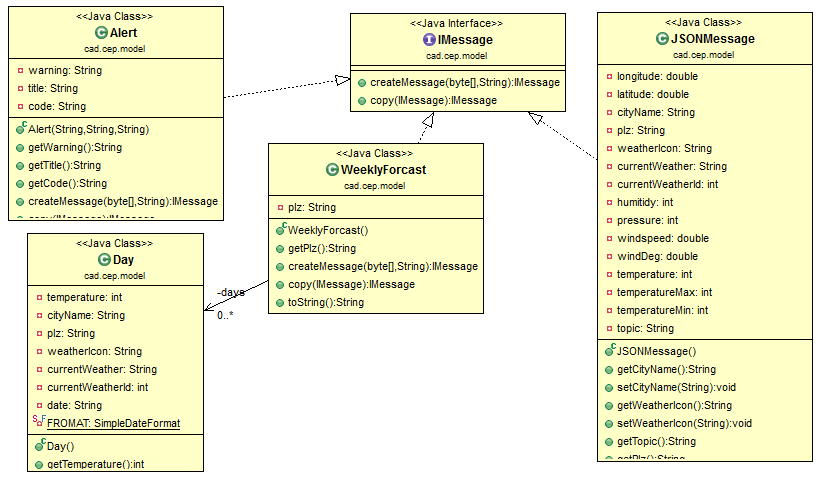
\includegraphics[width=0.5\textwidth]{Bilder/News.png}
	\caption{Das Klassendiagramm der Nachrichten}
	\label{img:eventDiagramm}
\end{figure} 
Sollte die CEP Engine etwas finden wird ein Alert gesendet. Diese Nachrichten beinhalten einen Titel, eine Warnung und einen Warnungscode. Der Title kann verwendet werden um rauszufinden worüber gewarnt wird, die Warnung selbst ist der englische default Text und der Code kann verwendet werden um die Warnung in eine andere Sprache zu übersetzen.  Die Folgende Tabelle Zeigt die Warnungcodes. 
\begin{table}[!ht]
  \centering
    \begin{minipage}{15cm}
      \centering
      \begin{tabular}{*{3}{|l|p{5.0cm}|p{5.0cm}}}\hline
      \multicolumn{4}{|c|}{\cellcolor[RGB]{200,200,200}Die Wanung-Codes} \\\hline
     \textbf{Code}&\textbf{Bedeutung}\\\hline
    T1&Tropisches Wetter: Luftfeuchtigkeit über 90\\
      \hline
     W1&Forstchance: Es kann sein das es Frost auf der Straße gibt\\
     \hline
     W2&Starke Kälte: Die Temperatur ist unter -9 Grad\\
     \hline
     W3&Starker Schneefall: Besonderst heftiger Schneefall\\
     \hline 
     S1&Gutes Wetter: Es scheint die Sonne und es hat über 25 Grad\\
     \hline
      H1&Herzinfakt Warnung: Für Herzkranke starke Luftdruck schwankungen\\
     \hline
      H2&Herzinfakt Warnung: Für Herzkranke zu hohe Temperatur (>=25)\\
     \hline
      \end{tabular}
   \caption{Die Wanung-Codes}\label{tab:WaningCodes}
    \end{minipage}
\end{table}
Die CEP Engine wird über die Klasse Engine Control gesteuert. Diese Singleton-Klasse geht sicher das die anderen Klassen zugriff auf von ihnen benötigten Fuktionen der Eingine haben aber dabei nicht mehr zugriff als Notwendig erhaltent. Die Klasse ist ein Singleton um sicherzugehen das jede Klasse auf die gleiche Engine zugreift. Die Klasse selbst erstellt eine Instanz der Klasse EsperService. Die Instanz wrid über eine Factory erstellt. Die Factory geht sicher das jedes benötigte Statement mit einen Listener verknüpft wird. Die EsperService-Klasse beinhaltet die tatsächliche Esper Engine und stellt einen Wrapper für diese dar. Das folgende Klassendiagramm zeigt die Methoden und die Abhängigkeiten der Klassen.
 \begin{figure}[htbp]
	\centering
	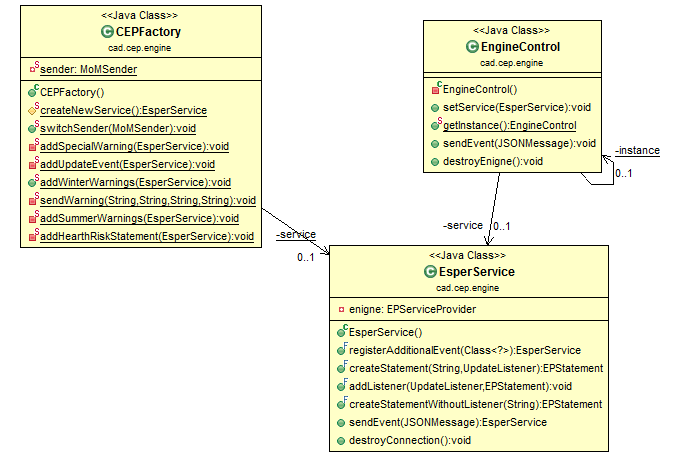
\includegraphics[width=0.5\textwidth]{Bilder/Esper.png}
	\caption{Das Klassendiagramm der CEP Klassen}
	\label{img:esperDiagramm}
\end{figure} 
Die Esper Statements sorgen dafür das Muster in den eingehenden Wetterdaten erkannt werden und reagieren mit passenden Nachrichten auf diese. Die Statements werden von der CEPFactory der Engine hinzugefügt. Jede eingehende Nachricht wird von midestens einen Statement erfasst. Der Entsprechende Listener sorgt dafür das die Clients die Daten erhalten und gibt eine Ausgabe aus. Zusätzlich werden die Daten in der Datenbank gespeichert. Dabei gibt es kein Fenster oder Consumption Mode. Jede Nachricht wird von diesen Statement erfasst und es dürfen auch weitere Statements greifen. Das Statement sieht wie folgt aus: 
\begin{lstlisting}
select * from JSONMessage
\end{lstlisting}
Ein weiteres Statement prüft ob die Luftfeuchtigkeit zu hoch ist. Bei einer hohen Luftfeuchtigkeit liegen tropische Verhältniesse vor, welche in Deutschland eher ungewöhnlich wären. Da alle unsere Wetterdaten aus Deutschland stammen ist es daher wichtig die Clients über eine solche besonderheit zu informieren. Auch dafür gibt es kein Fenster und keinen Consumption Mode. Treten die Bedingungen ein, liegt also eine Luftfeuchtigkeit von über 90 vor, wird ein Alert gesendet. Es dürfen aber auch andere Ereignisse ausgewertet werden.  Die Nachricht erhält den Code T1. 
\begin{lstlisting}
select * from JSONMessage where humidity >= 90
\end{lstlisting}
Einige Warnungen sind vorallen im Winter wichtig. Dabei geht es um Schneefall, niedrige Temperaturen und Frost. Die erste Winternachricht W1 warnt über eine Frostgefahr. Dabei werden zwei JSONMessages ausgewertet ob sie nacheinander ins System gekommen sind, dabei aus dem gleichen Ort stammen und Temperaturen unter 0 Grad angeben. Es werden zwei aufeinander folgende Nachrichten benötigt, da Wasser nicht sofort gefriert sondern Zeit braucht. Wenn also zwei Messungen eine neagtive Temperatur angeben, hatte das Wasser Zeit zu gefrieren. Sollte auf eine Nachricht mti negativer Temperatur eine Nachricht mit positiever Temperatur oder 0 Grad folgen, wird davon die erste Nachricht entfernt da das Wasser nicht genug zeit zum gefrieren hatte. Das Statement sieht wie folgt aus: 
\begin{lstlisting}
select * from pattern[m1=JSONMessage ->
m2=JSONMessage
(m1.plz = m2.plz and m1.temperature <0 and m2.temperature <0]
\end{lstlisting}
Über die Identifier m1 oder m2 können die einzelnen Nachrichten im Listener angesprochen werden. Der Listener sendet die Nachricht wieder als Alert weiter. W2 ist die zweite Nachricht und gibt eine Meldung bei besonderst kalten Temperaturen aus. Dabei benötigt es nur eine Nachricht mit einer Temperatur von unter -9 Grad um eine Warnung auszugeben. Niedirgere Temperaturen sind normalerweise selten in Deutschland und generell eher gefährlich. Daher muss eine Warnung an die Clients weitergeben werden. Das Statement funktioniert wie die bereits beschriebenen Statements. 
\begin{lstlisting}
select * from JSONMessage where temperature <=-9
\end{lstlisting}
Die Letzte Winternachricht befasst sich mit starken Schneefall. Dabei wrid der Wettercode von der Wetterapi ausgewertet. Der Code 622 bedeutet starker Schneefall. Die Clients können den Code zwar auswerten und auch entsprechend Meldungen ausgeben aber starker Schneefall kann gefährlich werden. Daher wird eine Meldung weitergesendet um sicherzugehen das alle Clients auch ihre Nutzer warnen. Das Statement sieht wie folgt aus. 
\begin{lstlisting}
select * from JSONMessage where currentWeatherId = 622
\end{lstlisting}  
Für den Sommer gibt es eine eigene Warnung. Diese warnt den Nutzer vor sehr guten Wetter. Das ist normalerweise nicht gefährlich aber es kann Clients interessieren ob sie ihren Nutzern sagen können, dass diese Baden gehen können. Dabei wurden als Bedingungen eine Temperatur über 25 Grad und ein klarer Himmel verwendet. Die ID dieses Alarms ist S1. 
\begin{lstlisting}
select * from JSONMessage where temperature > 25 and currentWeatherId >= 800
\end{lstlisting}
Die letzte Warnungskategorie beschäftigt sich mit Herzinfaktrisiken. Die Anwendung ist keine Medizinische Anwendung und folgt auch nicht den denentsprechenden Richtlinien. Daher kann die Anwendung nicht eine genaue Aussage darüber treffen ob ein Herzkranker Tabletten nehmen muss. Die Anwendung kann aber Aussgaben darüber treffen was laut Statistiken gefährlich für Menschen mit Herzproblemen werden könnte. Das stellt aber keine Empfehlung Medikamente zu nehmen dar. Es soll die Nutzer nur darauf hinweisen das sie sich Gedanken machen sollten, ob sie davon betroffen werden können. 
 Schwankt der Luftdruck zu strark, kann bei einigen Menschen es zu einen Herzinfakt kommen. Daher gibt es ein Statement welches überprüft ob in den letzten 30 Minuten eine starke Schwankung stattgefunden hat. Wenn eine Meldung in den Eventstream gelangt wird diese aufbewahrt bis das Zeitfenster abgelaufen ist oder das Muster erkannt wurde. Das Statement sieht wie folgt aus:

\begin{lstlisting}
select * from pattern[d1=JSONMessage ->
d2=JSONMessage
(p1.plz = p2.plz and
 (p2.pressure - p1.pressure <-5 or 
p1.pressure - p2.pressure <-10))
 where timer:within(30 min)]
\end{lstlisting} Das Statement W2 beschäftigt sich mit der Gefahr einer zu hohen Temperatur. Sollte diese über 25 Grad sein kann es in eingien Fällen das herzinfaktrisiko erhöhen. Das Statement dazu entspricht den anderen Updatestatements. 

\begin{lstlisting}
select * from JSONMessage wgere temperature >=25
\end{lstlisting}
 Zu jeden Eintrag in der Tabelle \ref{tab:WaningCodes} gibt es ein eigenes Statement. Dazu gibt es ein Statement um jede Nachricht zu erfassen. Dabei werden keine unique Consumptionmodes verwendet da eine Nachricht mehrere Statements auslösen kann. Es kann zum Beispiel gutes Badewetter, ein hoher Luftddruck und eine hohe Luftfeuchtigkeit gleichzeitig eintreten. Genauso wie eine Nachricht nicht im Eventstream bis zum erreichen eines Fensterendes oder eines Musters blockiert werden kann. Während die erste Nachricht darauf wartet wegen der temperatur Schwankungen festgehalten zu werden, kann eine andere Nachricht eingehen die in Kompination mit der ersten Nachricht ein anderes Muster erfüllt.  
\subsection{Ablauf}
Sobald die Anwendung gestartet wurde, ließt diese alle ihr bekannten Städte aus. Für jede Postleitzahl werden zwei Reader-threads erstellt. Einer davon wartet auf alle Nachrichten unter den Topic plz/today und der andere wartet auf alle Nachrichten unter dem Topic plz/weekly. Damit der Reader die Nachrichten auch erhält muss eine Verbindung zur MoM erstellt werden. Dafür wird die Adresse und die Credentials für die MoM aus den Umgebungsvariablen ausgelesen. Die Nachrichten kommen in einen JSON Format an. Dieses Format wird versucht in eine Instanz der Klasse JSONMessage umzuwandeln. Klappt das nicht wird verscuht daraus eine WeeklyForcast Nachricht zu machen. Klappt das auch nicht gibt die Anwendugn eine Fehlermeldung aus und ignoriert die Nachricht, Jede JSONMessage wird als Event den Eventstream der CEP weitergegeben. Sollte die Engine eine Besonderheit finden wird eine Warnung an plz/alert gesendet. Auf jedenfall wird die Nachricht an plz/today/cep weitergeleitet. Die Wochenvorhersage wird an plz/weekly/cep gesendet.  
\subsection{Erfüllte Anforderungen}
Die Anwendung muss sich natürlich an die Anforderungen des 12-Faktor App Standards halten. Die erste Anforderung Codebase wird dadurch erfüllt das die Anwendung selbständig und alleine Funktionieren kann. Die anderen Komponenten, wie zum Beispiel die Wetter API sind nicht notwendig. Sie wurden nur mit entwickelt um ein Vollständiges Scenario darstellen zu können. Die einzige notwendige andere komponente ist eine MoM. Dabei kann die MoM aber jederzeit ausgetauscht werden. Die MoM wurde auch nicht von uns entwickelt sondern nur auf dem Server aufgesetzt. 
\\
Die Abhänigkeiten werden mit Maven verwaltet. Jede Benötigte Bibliothek wird einfach als Dependency hinzugefügt und diese wird, mit allen von dieser Benötigten Bibliotheken, runtergeladen und im Buildpath hinzugefügt. Neue Versionen oder Abhänigkeiten können einfach mit einer Zeile mehr in der Konfiguration hinzugefügt werden. Es wird nichts an Code Verwendet was nicht entweder von Java selbst kommt (Version 1.8) oder aus einer in Maven definierten Bibilothek vorhanden ist. Die Anwendung geht niemals davon aus das etwas implizit vorhanden ist.
\\
Die Addresse der MoM, der Nutzername und das Passworrt sind alle in Umgebungsvariablen festgelegt. Die einzige Konsigurationsdatei im Projekt ist die pom.xml. Diese hat aber mit der laufenden Anwendung nach dem erstellen des Builds nichts mehr zu tun. 
\\
Die Anwendung verwendet als anderen Service die MoM. Diese wird über eine API angesprochen. Die API ist allgemeingültig für jede MoM, sofern sie MQTT unterstüzt. Die Datenbank wird über eine selbstgeschriebene API angesprochen. Die Art der Datenbank kann über eine neue Klasse ausgetauscht werden, da über ein Interface die Datenbank angesprochen wird. Die Adresse kann auch ausgetauscht werden. 
\\
Der Relasebuild kann nur von Jenkins erstellt werden. Dieses erstellt alle zusätzlichen für eine veröffentlichte Version benötigten Datein. Jenkins erlangt den Code über das Github Repository. Zu den Dateien gehört unter anderen die Konfiguration für das Deployment auf der Cloud.
\\
Säntliche Daten werden nur kurzeitig von der CEP Engine gespeichert. Die Anwendung legt keine Files an welche länger als die Ausführungszeit auf dem Server vorhanden sind. Daten die nicht mehr vorhanden sind, werden auch nicht mehr aufgerufen. Die CEP kennt nur die Temporär gespeicherten Daten. jede Datei die nicht mehr gespeichert ist, wird von der Engine nicht mehr berücksichtigt. Daher wird jede eingehende Nachricht zusätzlich in einer Datenbank gespeichert. Wenn die Engine startet werden alle Daten der letzten 24 Stunden geladen und neu gesendet. Auf dieseweise gehen keine Informationen verloren.
\\
Die Anwendung braucht nur eine JVM zum Laufen. Ansonsten wird davon ausgegangen das über die Cloud Foundry oder die Cloud eines anderen Anbieters über eine Einstellung die Anwendung mit einen Port verknüpft werden kann. 
\\
Es werden verschiedene Threads verwendet. Diese werden aber nicht wegen der zum skalieren verwendet, sondern um sicherzugehen das eine Nachricht ausgewertet werden kann während eine andere gesendet wird. Es soll also nur die Ausführungszeit verschiedener nebenläufig ausführbarer Schritte optimiert werden. Weitere instanzen der Cloud werden zum skalieren erstellt. 
\\
Es macht keinen unterschied ob die Anwendung normal geschlossen wurde oder abgestürzt ist. Die CEP Engine und die MoM Verbindung werden geschlossen und können ohne Probleme wieder geöffnet werden. Wenn eine Verbindung wieder gebraucht wird, wird diese automatsich wieder geöffnet. Nur die bisherigen Muster gehen Verloren wenn die Anwendung plötzlich abstürtzt. Sobald die Anwendung neu startet werden die Daten der letzten 24 Stunden geladen und neu gesendet. Die Muster können so wiederhergestellt werden. Alles was älter als 24 Stunden ist, ist nicht mehr relevant. 
\\
Es werden keine Log-Dateien angelegt. Die Anwendug gibt Mledungen über den Output- und den ErrorStream aus. An einer anderen Stelle muss daraus ein Log oder eine sonstige Auswertung erfolgen. 
\\
In der folgenden Tabelle werden die Anforderungen nochtmal zusammengefasst dargestellt. 
\begin{table}[!ht]
  \centering
    \begin{minipage}{15cm}
      \centering
      \begin{tabular}{*{3}{|l|p{5.0cm}|p{5.0cm}}}\hline
      \multicolumn{4}{|c|}{\cellcolor[RGB]{200,200,200}Validierung nach "12 Faktor APP"} \\\hline
     \textbf{ID}&\textbf{Anforderung}&\textbf{Validierungs Element}&\textbf{Erfüllt}\\\hline
     1.&Codebase&Andere Komponenten sind nur für das Testszenario da. Deployment verschiederner Versionen über Repo möglich&Ja\\
      \hline
     2.&Abhängigkeiten&Abhängigkeiten werden über Maven verwaltet&Ja\\
     \hline
     3.&Konfiguration&Bis auf Buildconfigurations gibt es keine Konfigurationsdatei. Alles andere über Umgebungsvariablen&Ja\\
     \hline
     4.&Unterstützende Dienste&Die unterstüzenden Dienste können über Umgebungsvariablen ausgetauscht werden&Ja\\
     \hline 
     5.&Build, release, run&Wird von Jenkins verwaltet&Ja\\
     \hline
     6.&Prozesse&Es gibt keine langfristig gespeicherten Daten&Ja\\
     \hline
      7.&Bindung an Ports&Wird von Cloud Foundry übernommen&Ja\\
     \hline
      8.&Nebenläufigkeit&Es wird nicht mit threads skaliert sondern mit Cloud Foundry instanzen&Ja\\
     \hline
      9.&Einweggebrauch&Verbindungen können beliebig geschlossen oder geöffnet werden ohne das wichtige Daten verloren gehen&Ja\\
     \hline
     10.&Dev-Prod-Vergleichbarkeit&Nicht zutreffent&Nein\\
     \hline     
     11.&Logs&Es wird mit den Streams gearbeitet.&Ka\\
     \hline
     12.&Admin-Prozesse&Nicht zutreffent&Nein\\
     \hline
      \end{tabular}
   \caption{Validierung der CEP nach "12 Faktor APP"}\label{tab:AnforderungenCEP}
    \end{minipage}
\end{table}
\section{Anwendersicht}
Für die Anwendersicht wurden zwei Applikationen erstellt. Zum einen eine Mobile Applikation und zum anderen eine Web Applikation. Die Mobile Applikation wurde für das Betriebssystem Android in AndroidStudio entwickelt. Die Web Applikation wurde mit Hilfe eines Bootstrap Templates erstellt. Beide Applikationen verwenden die Bibliothek Paho um mit der MOM zu Interagieren.  
\subsection{Android-App}
Die Android Applikation soll eine Wetter Applikation sein, dafür soll sie verschiedene Wetterdaten anzeigen können. Dazu wurde zu beginn des Projektes festgelegt, welche Daten anzeigt werden sollen. Diese können in zwei Kategorien unterschieden werden. Zum einen das \textbf{Tageswetter} und zum anderen die \textbf{Wochenvorhersage}. Unter das Tageswetter fallen die folgenden Punkte: 
\begin{itemize}
\item das Tageswetter als großes Icon
\item die momentane Temperatur in $^\circ$C
\item das genaues Wetter in Wörtern
\item der Standort
\item das Datum mit Uhrzeit
\item die Windgeschwindigkeit in km/h
\item die Windrichtung mit Hilfe einer grafischen Anzeige
\item die Regenwahrscheinlichkeit in \%
\end{itemize}  
Bei der Wettervorhersage für eine Woche ergeben sich nachfolgende Punkte
\begin{itemize}
\item die Wochentage ab dem Nachfolgetag des Tageswetters
\item ein kleines Wettericon
\item die Tagesmaximaltemperatur in $^\circ$C mit der Schriftfarbe rot
\item die Tagesminimaltemperatur in $^\circ$C mit der Schriftfarbe blau
\item ein Diagramm das die Maximal- und Minimaltemperaturen veranschaulicht
\end{itemize}  
Des Weiteren sollte es eine Auswahlmöglichkeit geben zwischen der Automatischen Standortbestimmung mittels GPS und der Eingabe einer Postleitzahl um den Standort festzulegen.
\begin{figure}[htbp]
	\centering
	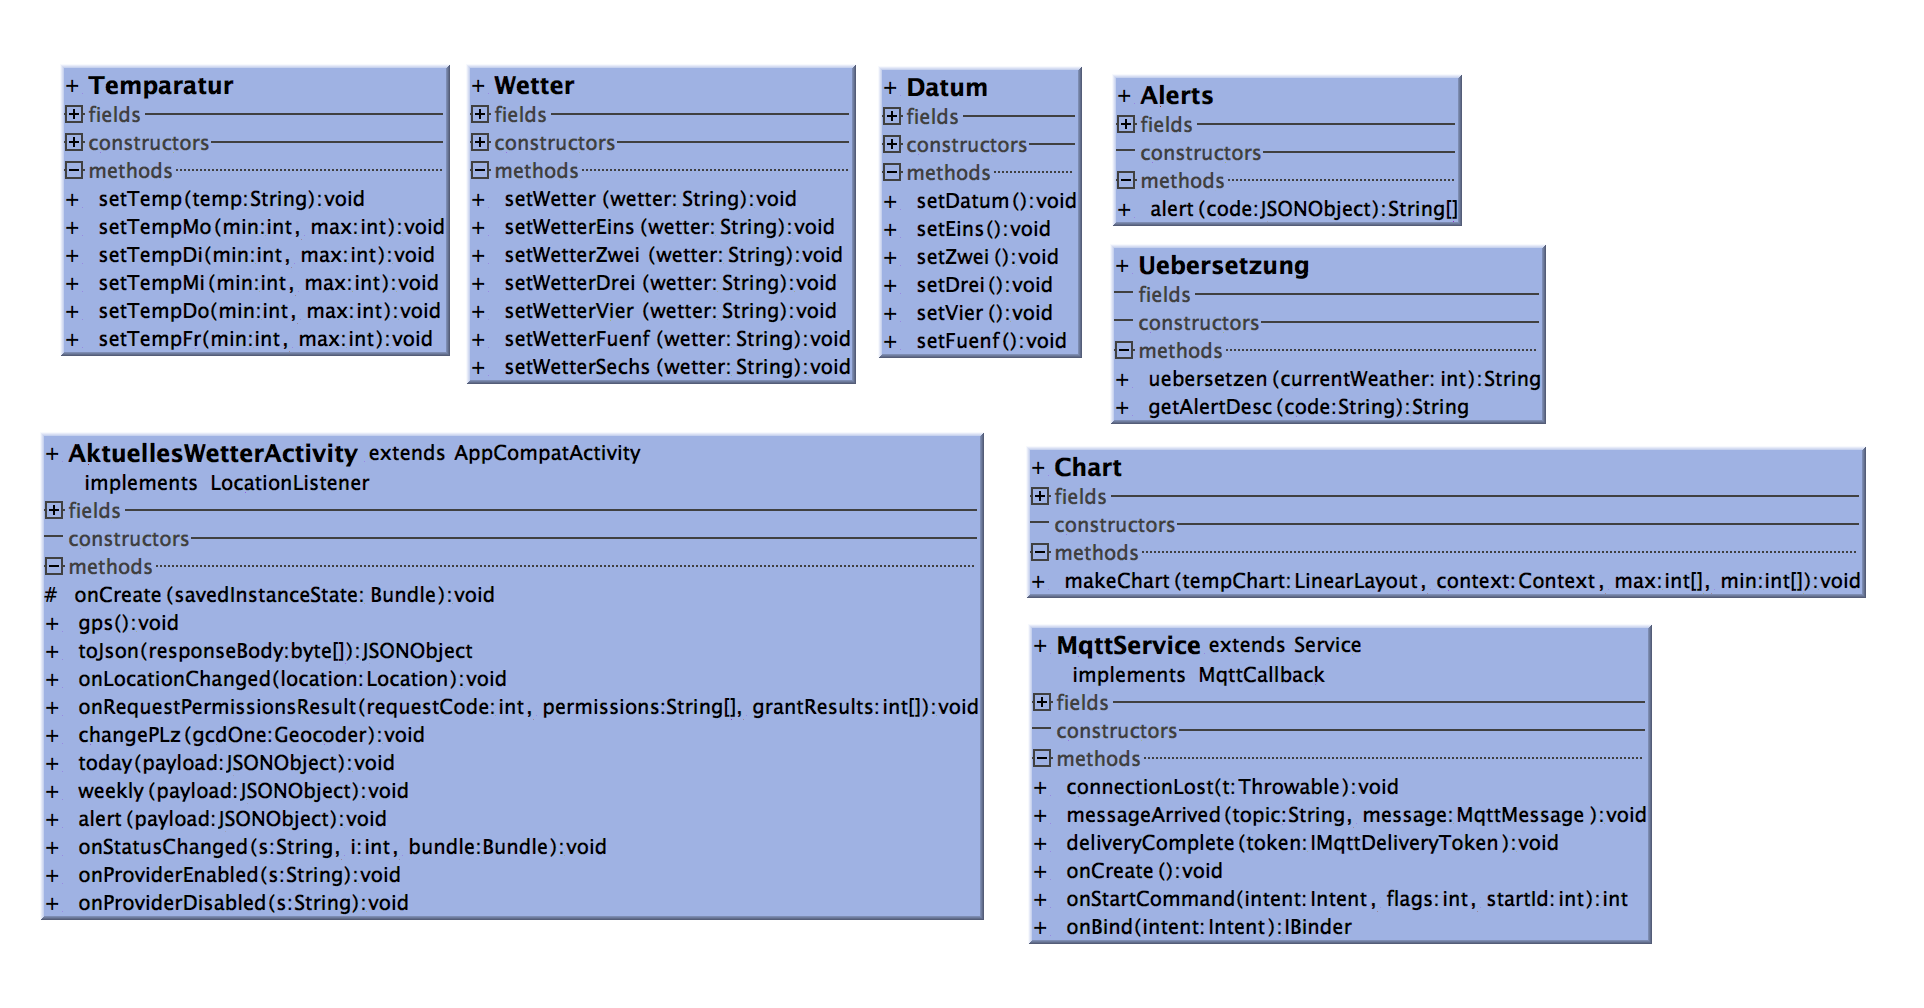
\includegraphics[width=1.0\textwidth]{Bilder/AndroidUML.png}
	\caption{Klassendiagramm der Android-Applikation}
	\label{img:AndroidUMLDiagramm}
\end{figure} 
Die Applikation wurde in Androidstudio in der Sprache Java und XML geschrieben. 
Aufgebaut ist die Applikation über 8 Klassen wie in  Abb. \ref{img:AndroidUMLDiagramm} zusehen ist. Die Klasse \textbf{AktuellesWetterActivity} fungiert dabei als Main-Class.
Die Klasse \textbf{MqttService} ist ein Android Service. Als einen Android Service bezeichnet man einen Prozess der nebenläufig zum Hauptprozess läuft. Dieser Service ist für die Verbindung zur MOM notwendig und wird später im Unterkapitel \ref{subsubsec:MqttService} näher erläutert.
Die weiteren Klassen sind Hilfsklassen zur Verarbeitung der, durch die MoM bereitgestellten Daten.
Beispielsweise übersetzt die Klasse \textbf{Uebersetzung} die verschiedenen Wettercodes in, für den Anwender lesbare, Wetterbezeichnungen. Dies geschieht mit Hilfe einer einfachen Switch-Case-Anweisung, wie exemplarisch in Abb. \ref{img:Case-Uebersetzung} zu sehen.
  \begin{lstlisting}
 switch (code) {
            case "H1": {
                return "Starke Luftdruckschwankungen, nehmen Sie Ihre Medizin falls benoetigt";
            }
            case "H2": {
                return "Temperaturen ueber 25 $^\circ$C, nehmen Sie Ihre Medizin falls benoetigt";
            }
            case "S1": {
                return "Ideales Badewetter";
            }
            case "W1": {
                return "Achtung, Frostgefahr";
            }
            case "W2": {
                return "Achtung, sehr niedrige Temperaturen. Ziehen Sie sich warm an.";
            }
            case "W3": {
                return "Achtung, schwere Schneefaelle.";
            }
            case "T1": {
                return "Luftfeuchtigkeit ueber 90%";
            }
        }
	\label{img:Case-Uebersetzung}
\end{lstlisting} 

Bei beginn der Applikation soll, wie in den Anforderungen beschrieben, die Position automatisch durch GPS ermittelt werden. Dazu wurde das von Android bereitgestellte Interface LocationListener verwendet. Dazu müssen die Methoden onLocationChanged(), onProviderDisabled(), onProviderEnabled() und onStatusChanged() implementiert werden. 
Die wichtigste Methode dabei ist die onLocationChanged(). Diese liefert jedes Mal wenn sich die Position des Smartphones verändert die neue Position zurück. 
Um nun das Interface LocationListener zu verwenden, ist es notwendig sich den Location Service bei den SystemServices zu holen. Dies geschieht über folgende Codezeile:
  \begin{lstlisting}
   LocationManager locationManager = (LocationManager) getSystemService(Context.LOCATION_SERVICE);
  \end{lstlisting}
  Des Weiteren ist es ab Android Version 6.0 (API Level 23) notwendig dem Anwender die Möglichkeit zugeben, die Standortbestimmung mittels GPS zu verweigern. Dafür muss eine Permissions Abfrage gemacht werden, welche von Android fertig bereitgestellt und in den Code eingebaut werden kann. Wenn das geschehen ist, kann über das Objekt locationManager die Methode requestLocationUpdates(String provider,long minTime, float minDistance, LocationListener listener) mit den Parametern: 
    \begin{itemize}
\item provider = "gps"
\item minTime = 10000 (Millisekunden)(dieser Wert ist für die App nicht so wichtig, da die Aktualisierung nur beim Start und auf Knopfdruck benötigt wird)
\item minDistance = 50 (in Meter)(dieser Wert ist für diese App nicht so wichtig, da die Genauigkeit der Position eine untergeordnete Rolle spielt)
\item listener = this (Klasse die das Interface LocationListener implementiert)
\end{itemize}  
aufrufen. Nachdem diese Methode mit den Settings des LocationManagers ausgeführt wurde, kann die Methode getLastKnownLocation("gps") der Klasse LocationManager aufgerufen werden. Diese Methode liefert ein Objekt der Klasse Location zurück. Dieses Location Objekt beinhaltet die Positionsdaten. Um nun von den Positionsdaten auf die benötigten Angaben wie Stadtname und Postleitzahl (PLZ) zukommen, wird ein Objekt der Klasse Geocoder benötigt. Die Klasse Geocoder ist ebenfalls Bestandteil der Android Location Library. Durch diese Klasse können die Längen- und Breitengrad Daten des Location Objektes in Stadtnamen und PLZ umgewandelt werden.
Liegen diese Daten vor kann der Stadtname auf der App angezeigt werden und der Android Service MqttService mit dem Übergabeparameter PLZ über folgenden Code 
 \begin{lstlisting}
private Intent serv = new Intent(this, MqttService.class);
serv.putExtra("plz", plz); 
startService(serv);
  \end{lstlisting}
gestartet werden.
\subsubsection{Mqtt Service}
\label{subsubsec:MqttService}
Der MqttService ist das Herzstück der Android Applikation in diesem Service wird die Verbindung zur MOM hergestellt und die Daten die diese liefert empfangen.
Mit dem Open Source Projekt Paho wurde eine Verbindung zu der in Kapitel \ref{rabbitmq} vorgestellten MOM realisiert. Dafür wurde die für Android spezifische Library über Grovy importiert. Durch diesen Import ist es möglich einen Android-Client zu erstellen. Dafür wurde das Interface MqttCallback implementiert. Zu diesem Interface gehören die Methoden: 
 \begin{itemize}
\item connectionLost(Throwable t):
\\Diese Methode hat den Zweck, wenn während des Betriebs der Applikation die Verbindung zur MOM verloren geht, diese wieder aufzubauen.
\item messageArrived(String topic, MqttMessage message):
\\In dieser Methode kommen die Messages der Abonnierten Topics als Byte Arrays und das dazugehörige Topic als String, zur Unterscheidung der Messages an.
\item deliveryComplete(IMqttDeliveryToken token):
\\Wird aufgerufen, wenn die Zustellung für eine Nachricht abgeschlossen ist und alle Bestätigungen eingegangen sind.
\end{itemize}
Wie im vorherigen Kapitel erwähnt wird der Service mit dem Parameter PLZ gestartet, dazu wird die Methode onStartCommand verwendet, diese besitzt als Aufrufparameter ein Intentobjekt, diesem wurde in der AktuellesWetterActivity ein "Extra" mit dem Key plz übergeben. Mit Hilfe dieses Keys kann der Übergebene Wert ausgelesen werden. Um nun eine Verbindung mit der MOM aufzubauen, werden vier Angaben benötigt. Diese sind zum einen die tcp-url und der Port der MOM. Zum anderen für die Authentifizierung bei der MOM einen Usernamen und ein Passwort. Der Username und das Passwort werden einem Paho ConnectionOption Objekt übergeben. Dabei wird das Passwort mittels eines Char-Arrays übergeben. Dieses ConnectionOption Objekt wird wiederum zusammen mit der Url, dem Port und einer Client-Id (diese wird automatisch erzeugt) an das eigentlichen Client Objekt übergeben. Dieses Client Objekt besitzt die Methode connect in dieser wird das Interface IMqttActionListener mit den Methoden onSuccess und onFailure aufgerufen. In der Methode onSuccess werden nun 3 Topics der MOM abonniert. Diese 3 Topics sind:
\begin{itemize}
\item plz/today/CEP:
\\ Liefert ein JSON Objekt mit dem Tages aktuellen Wetter für die Postleitzahl.
\item plz/weekly/CEP:
\\ Liefert ein JSON Array mit dem Wochenwettervorhersagen für die Postleitzahl.
\item plz/alert:
\\ Liefert ein JSON Objekt falls es eine Wetterwarnung für die Postleitzahl gibt.
\end{itemize}
Im Falle das eine Nachricht der MOM eintrifft wird, wird die weiter oben im Kapitel erwähnte Methode messageArrived aufgerufen.
Mit Hilfe eines BroadcastReceivers und einem weiteren Intentobjekts wird diese Nachricht an die AktuellesWetterActivity Klasse übergeben.
\subsubsection{Broadcast Receiver}
\label{subsubsec:BroadcastReceiver}
Ein Broadcast Receiver ist neben einem Activity und einem Service, eine weitere wichtige Komponente bei Android. Mit Hilfe eines BroadcastReceiver ist es möglich Nachrichten mit Hilfe eines Intentobjektes über Prozessgrenzen hinaus zu versenden. Ein BroadcastReceiver hat nur eine solange Lebensdauer wie es benötigt die erhaltene Nachricht zu bearbeiten. Ist diese Nachricht verarbeitet wird die Instanz des BroadcastReceivers beendet. Dies hat den Vorteil das der Akkuverbrauch des Smartphones gesenkt wird. Um einen BroadcastReceivers verwenden zu können muss dieser beim System mit einem Namen registriert werden, dies zeigt die nachfolgende Codezeile:
\begin{lstlisting}
 LocalBroadcastManager.getInstance(this).registerReceiver(broadcastReceiver, new IntentFilter("NOW"));
  \end{lstlisting}
Dieser BroadcastReceivers wurde mit dem Namen "NOW" registriert.
Innerhalb dieses Receivers wird nun die Ausgabe der Daten, die von der MOM gesendet wurden, geregelt. Dazu wird über das Topic entschieden wie mit der angekommenen Message verfahren wird (siehe nachfolgendes Codefragment).
\begin{lstlisting}
public void onReceive(Context context, Intent intent) {
            byte[] mes = intent.getByteArrayExtra("Message");
            Log.e("onReceive: ", new String(mes));
            if (new String(mes).contains("hallo")) {
            } else {
                JSONObject payload = toJson(mes);
                String topic = intent.getStringExtra("Topic");
                if (topic.contains("today")) {
                    today(payload);
                } else {
                    if (topic.contains("weekly")) {
                        weekly(payload);
                    } else if (topic.contains("alert")) {
                        alert(payload);
                    }
                }
            }
        }
  \end{lstlisting}
  
  Um nun das in den Anforderungen gewünschte Diagramm zu erzeugen gibt es die Klasse Chart. Diese erzeugt mit Hilfe der in Weekly enthaltenen Minimum- und Maximumtemperaturen für die einzelnen Tagen ein Liniendiagramm. Dazu wurde die free Library aChartengine verwendet.
Die nachfolgende Abb. \ref{img:AndroidApplikation} zeigt die fertige Applikation mit dem Tageswetter und der Wochenvorhersage.

\begin{figure}
    \subfigure{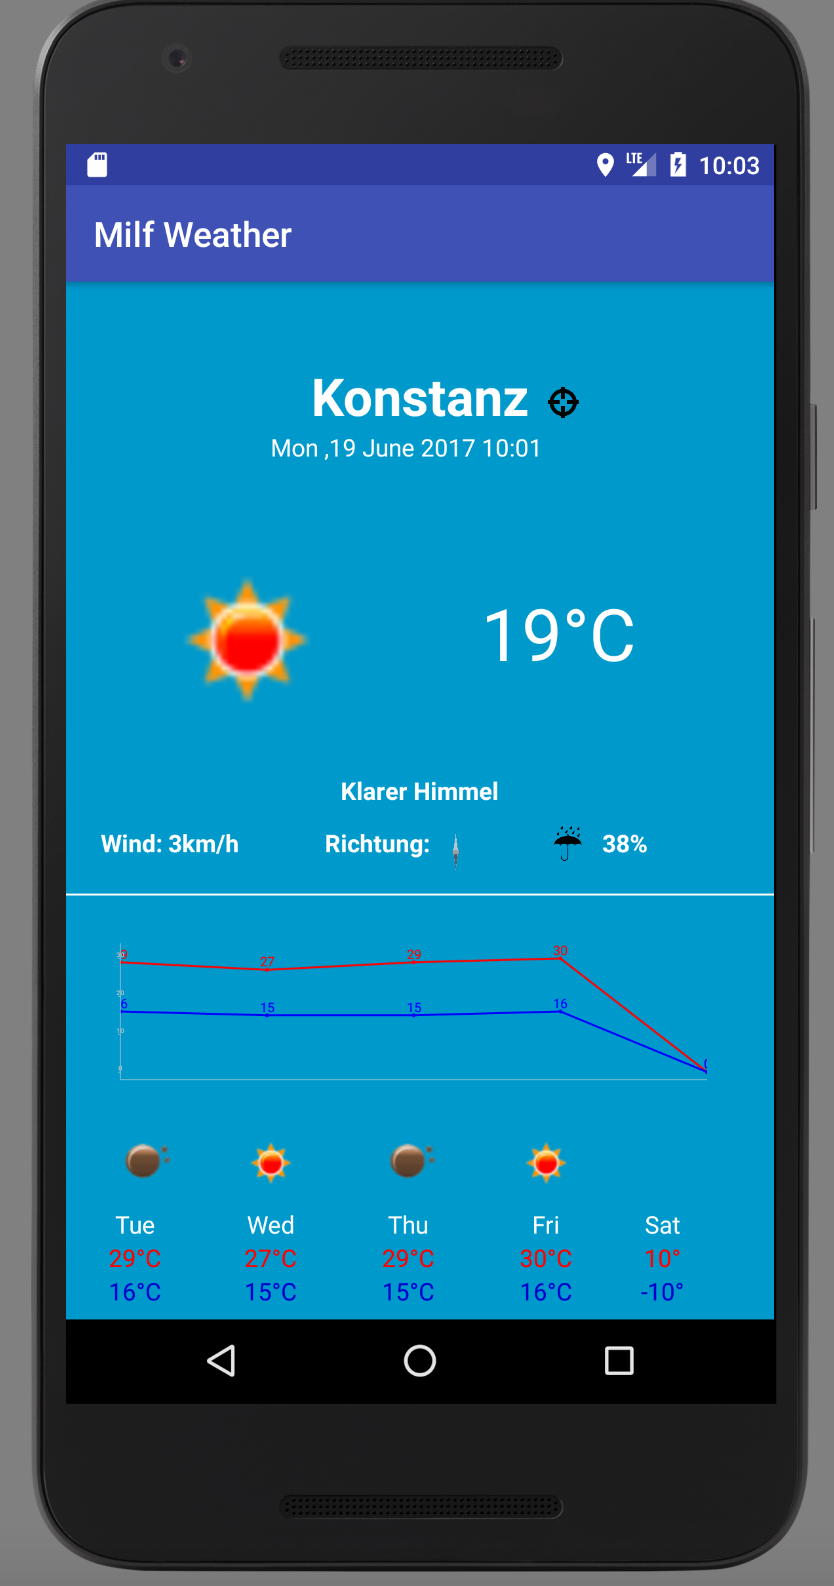
\includegraphics[width=0.5\textwidth]{Bilder/AndroidApp.png}}
    \subfigure{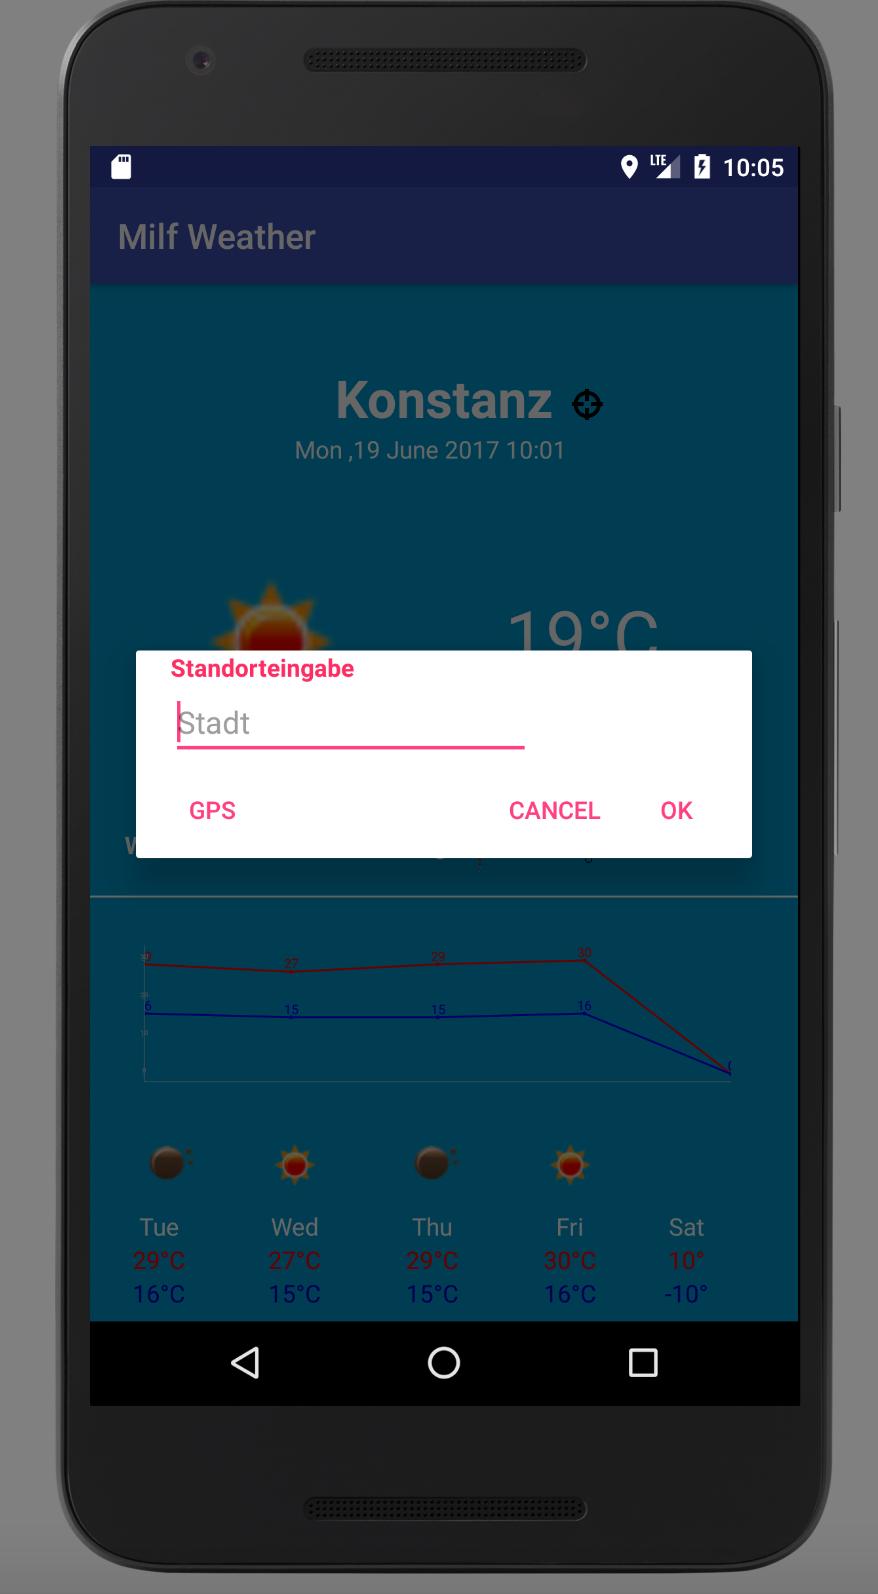
\includegraphics[width=0.5\textwidth]{Bilder/AndroidAppPLZ.png}}
\caption{Android-Applikation}
\label{img:AndroidApplikation}
\end{figure}


\subsection{Web-Client} \label{Web-Client}
Der Web-Client stellt dem Endnutzer eine Darstellung der Wetterdaten zur Verfügung. Die angezeigten Daten gleichen denen der Android-App, die Darstellungsform ist jedoch für größere Bildschirme optimiert. 
\subsubsection{Layout}
Das Layout der Applikation baut auf ein Template von Bootstrap auf und ist untergliedert in die Navigationsleiste am oberen Rand, einen sogenannten Jumbotron Container für das aktuelle Wetter, einem Block für die Vorhersage und schlussendlich einen Footer. 
\begin{figure}[htbp]
	\centering
	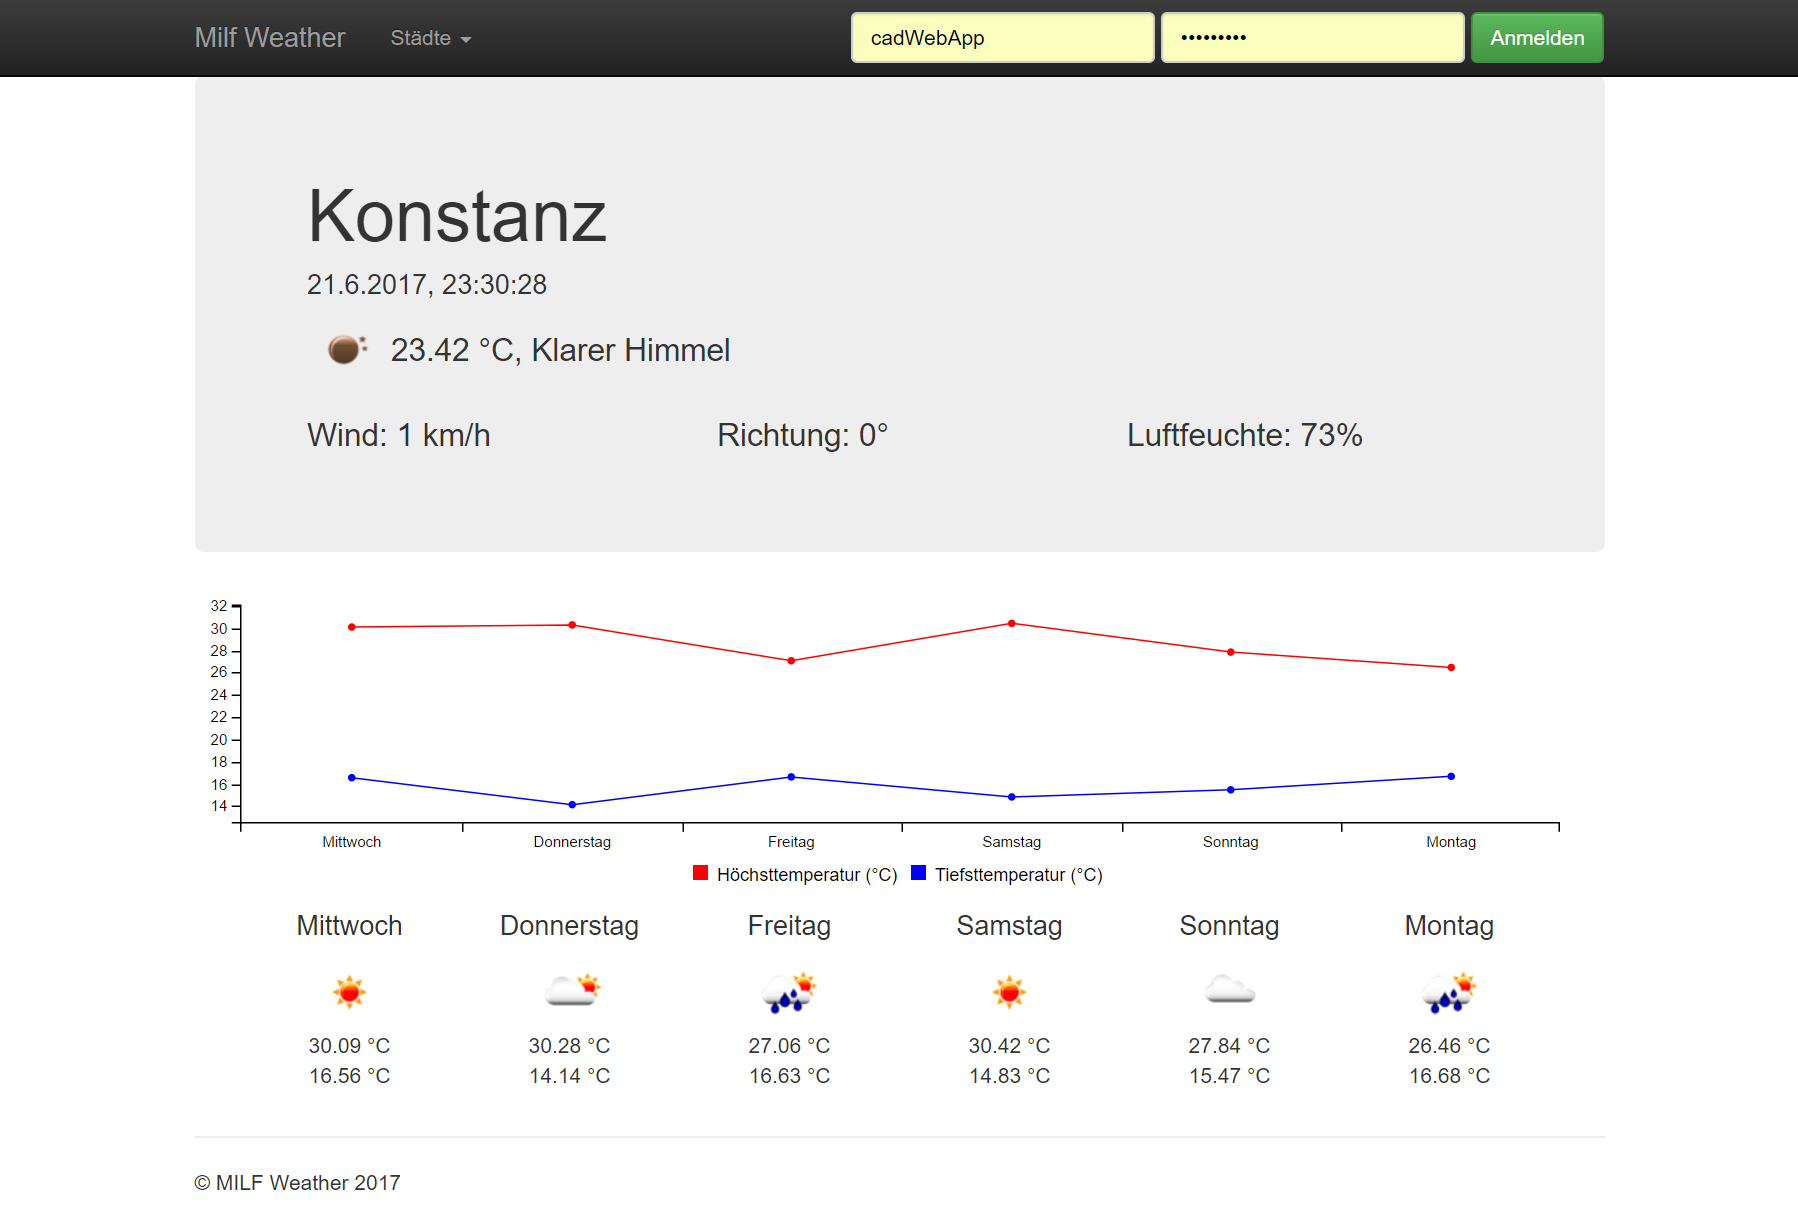
\includegraphics[width=1.0\textwidth]{Bilder/Web-Client.png}
	\caption{Web-Client}
	\label{img:webclient}
\end{figure}
Die Navigationsleiste enthält neben dem Seitennamen ein Dropdown-Menü, über welches die Auswahl der Stadt erfolgt, und ein Login Formular mit Eingabefeldern für den Benutzernamen und das Passwort sowie einen Button. Reicht der Platz zur Darstellung nicht aus, werden die Stadtauswahl und Loginmaske durch einen Button ersetzt, über den sich die Navigationsleiste ausfahren lässt um dann die Funktionen dort anzuzeigen.
Unterhalb der Navigationsleiste schließt ein farblich abgetrennter Bereich an, in dem prominent das aktuelle Wetter, der gewählte Ort sowie Datum und Uhrzeit dargestellt werden. Die Wetterdarstellung umfasst eine graphische Repräsentation in Form eines Icons, die aktuelle Temperatur in Grad Celsius, eine textuelle Beschreibung des Wetters sowie die Windgeschwindigkeit in km/h, die Windrichtung und die Luftfeuchtigkeit.
Anschließend wird die prognostizierte Höchst- und Tiefsttemperatur über den Wochentagen in einem Diagramm dargestellt und direkt darunter wird eine Wetterdarstellung in Form eines Icons sowie die Höchst- und Tiefsttemperatur textuell dargestellt.
Am Schluss der Webseite kommt ein Footer, der Platz bietet für rechtliche Informationen.

Technische Umsetzung
Auf technischer Seite nutzt die Webapplikation die Sprachen PHP, JavaScript, HTML und css. PHP wird ausschließlich verwendet um die Variablen, welche für die Verbindung zu Message Oriented Middleware benötigt werden, aus den beim Serverhost konfigurierbaren Umgebungsvariablen auszulesen, wie in Abb.\ref{img:Einbindung PATH-Variablen} zu sehen.
\begin{lstlisting} 
<script type="text/javascript">
  momAddress = "<?php echo getenv("momAddress"); ?>";
  momPort = "<?php echo getenv("momPort"); ?>";
  tenant = "<?php echo getenv("tenant"); ?>";
  topicToday = "<?php echo getenv("topicToday"); ?>";
  topicWeek = "<?php echo getenv("topicWeek"); ?>";
  topicAlert = "<?php echo getenv("topicAlert"); ?>";
</script>
\label{img:Einbindung PATH-Variablen}
\end{lstlisting}
Die Verbindung zur MOM wird clientseitig über die JavaScript Bibliothek Paho aufgebaut. Paho ist ein Projekt der Eclipse Foundation - bekannt vor allem für die gleichnamige IDE - mit dem Ziel Internet of Things Applikationen die Implementierung des MQTT Protokolls zu vereinfachen. Paho ist für eine ganze Reihe von Sprachen verfügbar, darunter Java, Python, C, C++ und dem hier verwendeten JavaScript. Der Funktionsumfang unterscheidet sich jedoch und so unterstützt die JavaScript Version nicht das Standard MQTT Protokoll, sondern nur eine angepasste Version für WebSockets. Für RabbitMQ lässt sich die Unterstützung von WebSockets über das RabbitMQ Web MQTT Plugin hinzufügen. Dies ermöglicht eine direkte Verbindung zwischen dem Browser des Nutzers und der MOM, ohne weitere Interaktion mit dem Webserver.
In Kombination mit der Umsetzung als Single Page Application bedeutet dies eine minimale Belastung des Webservers und erlaubt somit eine große Anzahl Nutzer pro Server. Bei Herokus kostenlosem Hostingmodell, welches nur 512 MB RAM und einen Worker bereitstellt waren so bereits in Tests über einen Zeitraum von einer Minute 1500 Aufrufe der Seite pro Sekunde möglich (vgl. Abb.\ref{img:testsettings} und \ref{img:testresults}.
\begin{figure}[htbp]
	\centering
	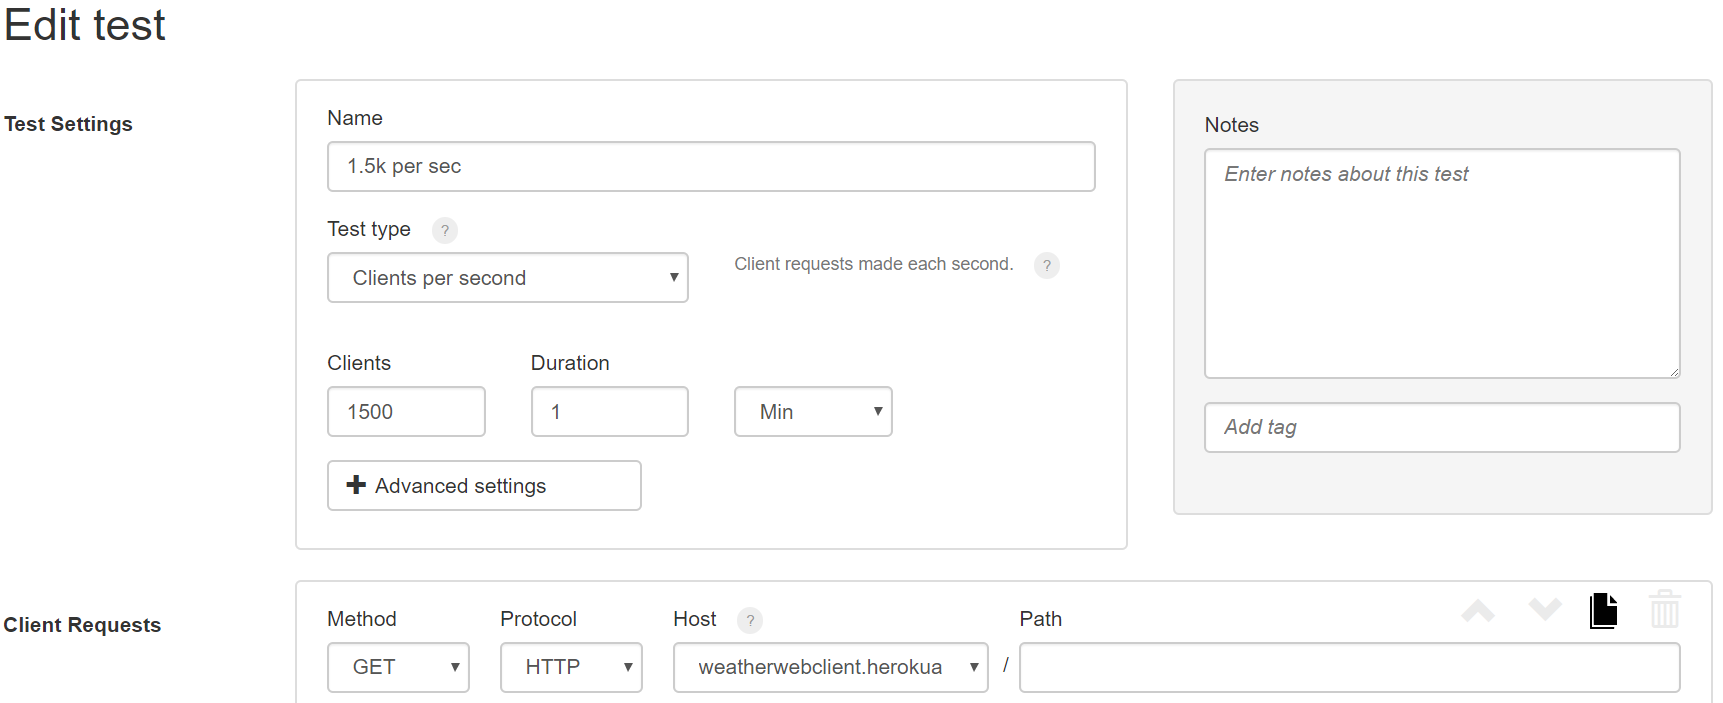
\includegraphics[width=1.0\textwidth]{Bilder/Web-TestSettings.png}
	\caption{Testeinstellungen}
	\label{img:testsettings}
\end{figure}
\begin{figure}[htbp]
	\centering
	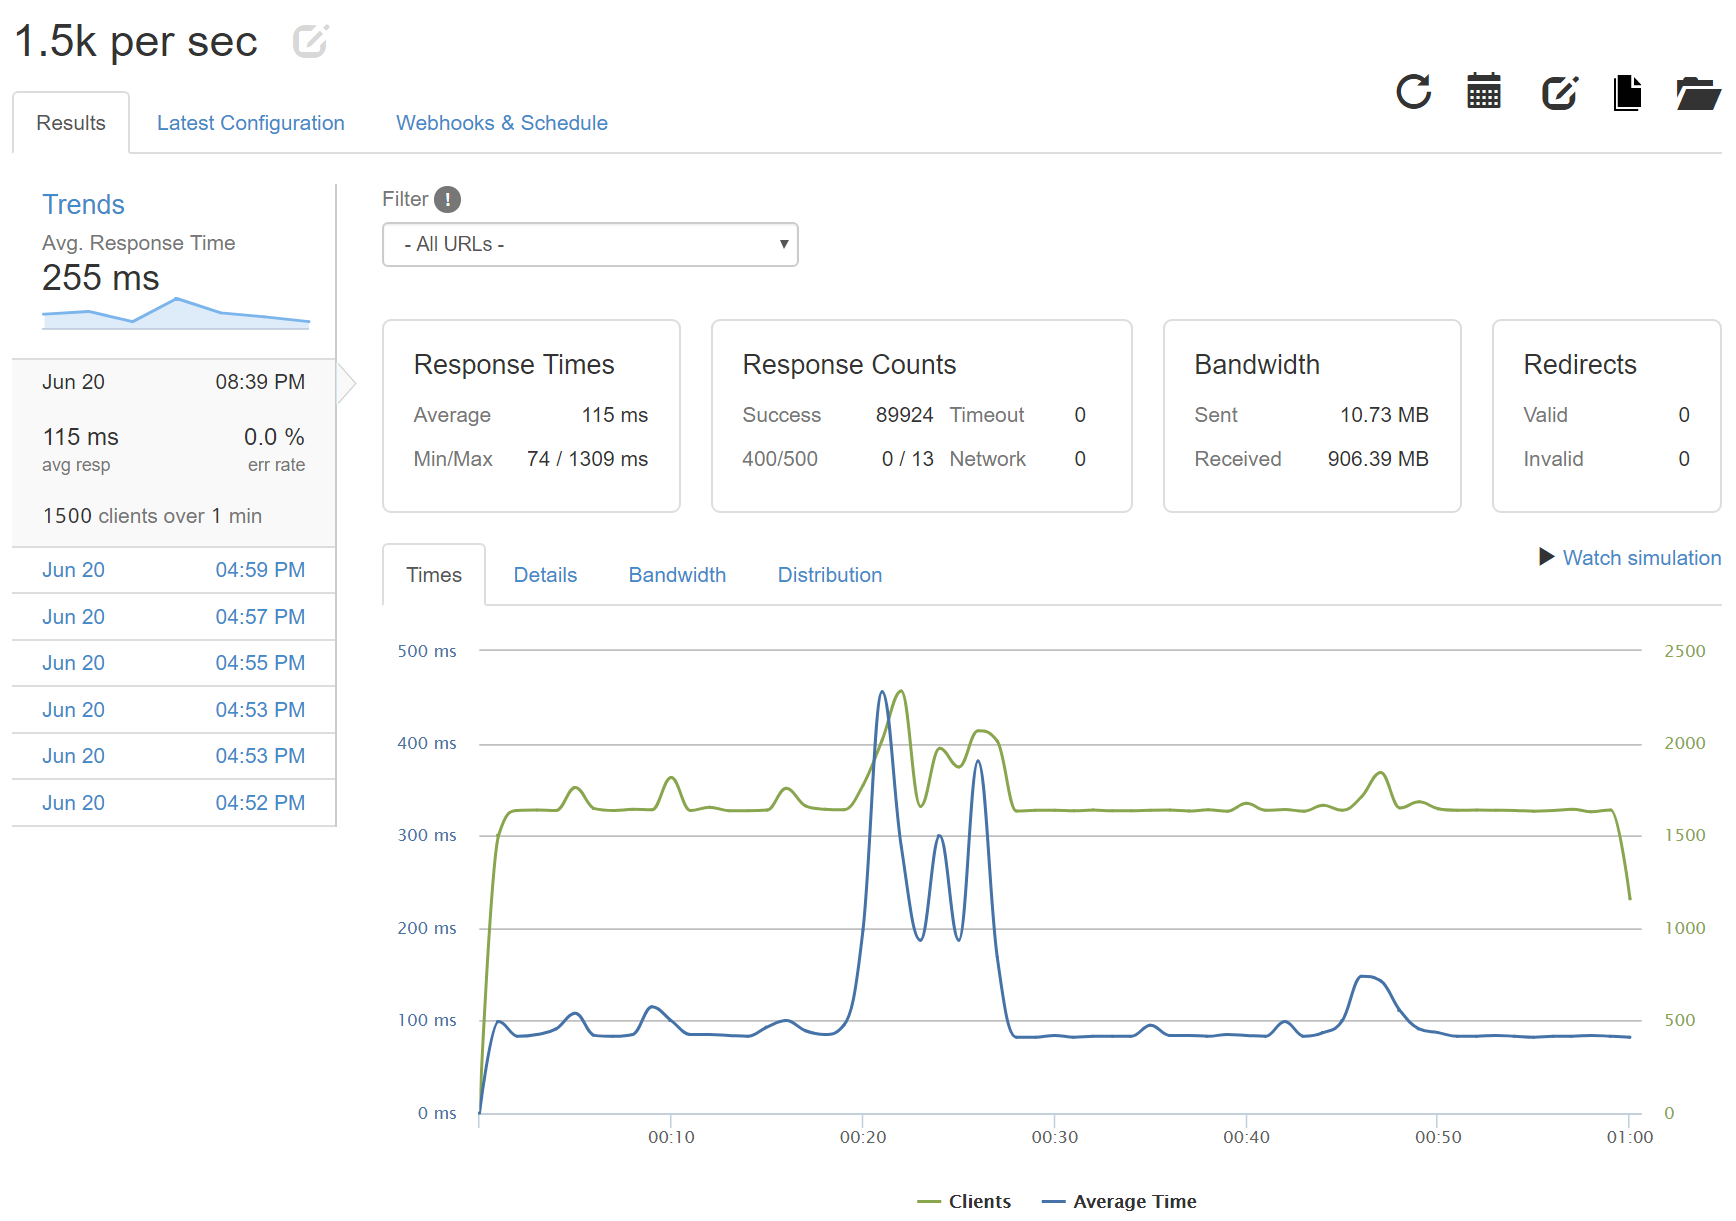
\includegraphics[width=1.0\textwidth]{Bilder/Web-TestErgebnisse.png}
	\caption{Testeinstellungen}
	\label{img:testresults}
\end{figure}
. Getestet wurde dies über den cloudbasierten Lasttest der SendGrid Labs, welcher unter der Webseite www.loader.io verfügbar ist und in einem AWS Rechenzentrum an der amerikanischen Ostküste läuft. 
Kommt der Benutzer auf die Webseite kann er eine Stadt wählen und sich einloggen. Der Login startet im JavaScript Code die Funktion connect und löst somit einen Verbindungsversuch zur MOM aus. Wurde beim Nutzername der Tenant nicht mit angegeben wird automatisch der Default-Tenant verwendet. Bei erfolgreicher Verbindung wird der Callback onConnect aufgerufen, der die Topics für das aktuelle Wetter, die Vorhersage und die Wetterwarnungen des gewählten Ortes abonniert. Geht zu einem Topic eine neue Nachricht ein wird diese in der Funktion onMessageArrived behandelt. Hierbei wird unterschieden zu welchem Topic die Nachricht gehört und im Fall des aktuellen Wetters oder der Vorhersage auch, ob die Nachricht neue Informationen enthält. Ist dies nicht der Fall wird die Nachricht nicht weiter behandelt, da dies an den dargestellten Informationen nichts ändern würde. Unterscheidet sich die Nachricht zur vorherigen wird die Nachricht dekodiert und die neuen Informationen werden mit Hilfe von jQuery-Funktionen in der HTML-Darstellung eingebunden, wie nachfolgend zu sehen ist. 
\begin{lstlisting} 
switch (message.destinationName) {
  case topicToday:
    //console.log("today: ", message.payloadString);
    todayData = message.payloadString;
    if (todayData != todayDataLast) {
      todayDataLast = todayData;
      var data = JSON.parse(todayData);
      $("#nowImage").attr("src", "img/" + data.weatherIcon + ".png");
      $("#nowTemp").text(data.temperature);
      $("#nowDescription").text(getWeatherDesc(data.currentWeatherId));
      $("#nowWindSpeed").text(data.windspeed);
      $("#nowWindDirection").text(data.windDeg);
      $("#nowHumidity").text(data.humidity);
      ...      
    }
    ...
}
\label{img:Verarbeiten-des-Topics-today}
\end{lstlisting}


Zur Generierung des Graphen (vgl. \ref{img:renderGraph}) wird die Bibliothek c3.js benutzt, welche wiederum intern d3.js verwendet, jedoch die Erstellung von Diagrammen mit weniger und einfacherem Quellcode ermöglicht als bei d3.js nötig wäre. Die erzeugten Graphen passen sich an die Anzahl, Minimal- und Maximalwerte der zu visualisierenden Daten an und skalieren mit der Bildschirmgröße. Die Konfiguration des Diagramms erfolgt über die Funktion generateGraph. Hier wird unter „bindto“ der css-selector angegeben, in dem der Graph erzeugt werden soll. Die Größe wird unter „size“ auf eine Höhe von 200 Pixeln begrenzt, unter „axis.x“ wird die Beschriftung entlang der X-Achse definiert. Entlang der y-Achse passt sich die Skala automatisch an die unter „data.columns“ eingetragenen Daten an. Die Datenpaare werden mit Höchst- bzw. Tiefsttemperatur benannt und farblich rot bzw. blau definiert. Über den Punkt padding wird der linke sowie rechte Abstand zum Container festgelegt. Hier muss genügend Platz für die Beschriftung links sein, da die Außenpunkte für die Darstellung der Start- bzw. Endpunkt der X-Achse ist. Um die schriftliche Vorhersage ausgerichtet unter dem Graphen darzustellen muss im css für diese der gleiche Abstand, jedoch als Margin, festgelegt werden.

\begin{lstlisting} 
// renders the graph
function generateGraph(data) {
  c3.generate({
    bindto: "#chart",
    size: {
      height: 200
    },
    data: {
      columns: [
        ["Hoechsttemperatur (Grad C)",
          data.days[0].temperatureMax, data.days[1].temperatureMax, data.days[2].temperatureMax,
          data.days[3].temperatureMax, data.days[4].temperatureMax, data.days[5].temperatureMax],
        ["Tiefsttemperatur (Grad C)",
          data.days[0].temperatureMin, data.days[1].temperatureMin, data.days[2].temperatureMin,
          data.days[3].temperatureMin, data.days[4].temperatureMin, data.days[5].temperatureMin]
      ],
      colors: {
        "Hoechsttemperatur (Grad C)": "red",
        "Tiefsttemperatur (Grad C)": "blue"
      }
    },
    axis: {
      x: {
        type: "category",
        categories: [
          getDayString(new Date(data.days[0].date).getDay()), getDayString(new Date(data.days[1].date).getDay()),
          getDayString(new Date(data.days[2].date).getDay()), getDayString(new Date(data.days[3].date).getDay()),
          getDayString(new Date(data.days[4].date).getDay()), getDayString(new Date(data.days[5].date).getDay())
        ]
      }
    },
    padding: {
      //same values as in main.css #weekDetails
      right: 30,
      left: 30
    }
  });
}
\label{img:renderGraph}
\end{lstlisting}

Wie der Graph, passt sich auch der Rest der Webseite dynamisch an die Anzeige des Nutzers an. Dies wird durch den Einsatz von Bootstrap erreicht. 

\subsubsection{12 Faktor App}\label{web12FactorApp}
In diesem Absatz wird in nachfolgender Tabelle dargestellt, ob und wie die Anforderungen der 12 Faktor App umgesetzt wurden.


\begin{table}[!ht]
  \centering
    \begin{minipage}{17cm}
      \centering
      \begin{tabular}{*{3}{|l|p{3.0cm}|p{7.0cm}}}\hline
      \multicolumn{4}{|c|}{\cellcolor[RGB]{200,200,200}Validierung nach "12 Faktor App"} \\\hline
     \textbf{ID}&\textbf{Anforderung}&\textbf{Validierungs Element}&\textbf{Erfüllt}\\\hline
     1. & Codebase & Codebase in git verwaltet, deployment verschiedener Versionen über Repo möglich & Ja\\
      \hline
     2. & Abhängigkeiten & Bibliotheken werden über CNDs aufgelöst und geladen, inklusive Fallback & Ja\\
     \hline
     3. & Konfiguration & Konfiguration \& Credentials werden über Umgebungsvariablen ausgelesen & Ja\\
     \hline
     4. & Unterstützende Dienste & MOM kann über Konfiguration ausgetauscht werden & Ja\\
     \hline 
     5. & Build, release, run & Push auf entsprechenden Git Branch löst einen Build \& und bei Erfolg ein Release aus & Ja\\
     \hline
     6. & Prozesse & Der Client läuft im Browser des Nutzers und serverseitig  müssen keine Daten verarbeitet/ gespeichert werden & Ja\\
     \hline
      7. & Bindung an Ports & Der Webserver wird nur zum Einlesen der Konfiguration verwendet, lokal kann über localhost oder sogar das filesystem zugegriffen werden & Ja\\
     \hline
      8. & Nebenläufigkeit & Die App verwendet bei Heroku Web- und Workerprozesse und kann horizontal skaliert werden & Ja\\
     \hline
      9. & Einweggebrauch & Die App kann jederzeit gestoppt und auch schnell wieder gestartet werden. Da der Nutzer keine aktive Verbindung zur App hält bekommt dieser davon nichts mit & Ja\\
     \hline
     10. & Dev-Prod-Vergleichbarkeit & Änderungen können vom Entwickler selbst binnen Sekunden deployed werden, zur Entwicklung wird der gleiche Webserver verwendet & Ja\\
     \hline     
     11. & Logs werden auf stdout geschrieben, von Heroku werden diese erfasst und zum abrufen bereitgestellt  & Ja\\
     \hline
     12. & Admin-Prozesse & Es werden keine Admin-Prozesse benötigt oder verwendet & nicht zutreffend\\
     \hline
      \end{tabular}
   \caption{Validierung der CEP nach "12 Faktor App"}\label{tab:AnforderungenCEP}
    \end{minipage}
\end{table}

\section{Deployment}
Das Deployment der einzelnen Komponenten erstreckt sich auf mehrere Plattformen. So werden die Wetter-Api und die CEP auf die Cloud Application Platform Cloudfoundry des Anbieters Pivotal deployed. Das Deployment des entwickelten Webclients erfolgt über Heroku und die Messaging Komponente RabbitMQ wird als Dockercontainer durch den Amazon Container Service deployed. Die Vorgehensweise bei den unterschiedlichen Anbietern wird in den nachfolgenden Absätzen vorgestellt.

\subsection{Cloudfoundry (Pivotal)}
Für das Deployment des Wetter-API Service und für die CEP wurde der Cloudanbieter Pivotal ausgewählt. Dieser Anbieter zeichnet sich durch ein großzügiges Angebot einer Testversion für welche keinerlei Zahlungsmittel hinterlegt werden mussten. Pivotal vergibt nach der Registrierung ein Guthaben von \$87. 

Für jede Komponente wurde ein extra Zugang in Pivotal angelegt, damit jede Komponente das volle Budget zur Verfügung hat, welches beim Testen der Skalierbarkeit benötigt werden wird. 

Zu Beginn des Projektes wurden die Komponenten manuell über das Terminal auf Pivotal hochgeladen. Da es sich bei beiden Komponenten um ein Maven-Projekt handelt, musste lediglich eine .jar oder .war aus der "pom.xml" erstellt werden, welche dann hochgeladen werden konnte. 

Folgende Befehle sind für ein manuelles Deployment des Wetterservice nötig: 

\begin{itemize}
\item mvn package, 
\item cf login, 
\item cf push wetterdata-cf-api -p mqtt-1.0.0.war.
\end{itemize}

Alle beschriebenen Befehle stehen unter der Annahme, dass sich im richtigen Verzeichnis aufgehalten wird. Analog dieser Befehle sehen die Befehle für ein manuelles Deployment der CEP aus, lediglich mit anderem Login und einer .jar. Bei beiden Deployments wurde auf eine Manifest-Datei verzichtet, die benötigten "env" wurden direkt in Pivotal hinterlegt. 

Da im weiteren Zuge des gesamten Projektes entschieden wurde auf "continuous deployment" zu bauen, wurde hierfür ein Jenkins-Server aufgesetzt. Dieser Jenkins-Server wird im Kapitel \ref{Jenkins} näher beschrieben. 

\subsection{Docker}\label{Docker}
Die in Absatz \ref{rabbitmq} erläuterte Message Oriented Middleware RabbitMQ wird als Docker Container deployed. Durch die Verwendung von Docker Containern ist es möglich, lauffähige Software in isolierten Containern zu starten. Dies hat den Vorteil, dass die Software immer in identischen Umgebungen gestartet wird, unabhängig davon ob der Container lokal auf dem Entwicklungsrechner oder auf dem Produktivsystem läuft. Dies betrifft auch die Abhängigkeiten von notwendigen Installationen. So basiert RabbitMQ wie in Absatz \ref{rabbitmq} erwähnt auf der Sprache Erlang, weshalb diese auf jedem Entwicklungs- und Produktivsystem installiert werden müsste. Durch die Verwendung von Docker können notwendige Installationen bereits im Dockerfile definiert werden. So wird beispielsweise die Installation von Erlang in Abb. \ref{img:erlangDockerfile} veranschaulicht. 

\begin{figure}[htbp]
	\centering
	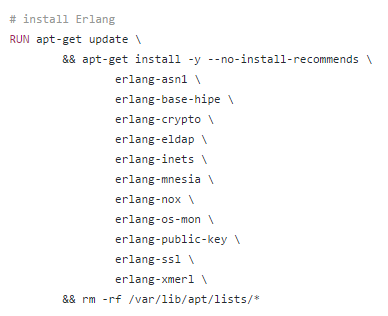
\includegraphics[width=0.5\textwidth]{Bilder/erlangDockerfile.png}
	\caption{Installation von Erlang im Dockerfile Quelle: https://github.com/docker-library/rabbitmq/blob/a6cb36022a5c1a17df78cfafe45a73d941ad4eb8/3.6/\-debian/Dockerfile}
	\label{img:erlangDockerfile}
\end{figure}
Dies ist ein Ausschnitt aus dem Dockerfile des offiziellen RabbitMQ-Baseimages, einer Abbildung des Containers. Der Abschnitt stellt die Installation von Erlang auf einem Linux-System unter Verwendung des Paketmanagers \textit{Advanced Packaging Tool} (APT) dar.
\subsubsection{Dockerfile}
Das Dockerfile für diesen Use-Case besteht neben dem erwähnten Baseimage aus Aktivierungen des in Absatz \ref{rabbitmq} vorgestellten Management Plugins, des MQTT Plugins sowie des MQTT-Websocket Plugins. Durch die Verwendung des Websocket Plugins ist die Kommunikation mit RabbitMQ auch über Webseiten möglich. Ein weiterer Bestandteil des Dockerfiles ist die rabbitmq.config. Diese ist notwendig um den Zugriff auf die MOM einzuschränken, da andernfalls eine Default-Konfiguration verwendet werden würde und durch diese der Nutzer \emph{guest} vollen Zugriff hätte. Um dennoch Administrations-Zugriff zu erlangen, wird über das Shell-Skript \textit{init.sh} ein Nutzer mit Administratorrechten angelegt. Die Zugangsdaten dieses Nutzers sind als Umgebungsvariablen hinterlegt. Die Ausführung des Skripts wird über den CMD-Befehl des Dockerfiles gesteuert. Zusätzlich ist es notwendig, Docker über den Befehl EXPOSE zu informieren, welche Ports der Container abhört. Im Anschluss an die Erstellung des Dockerfiles kann durch den Befehl \emph{docker build} ein Image erzeugt werden. Dieses Image wird auf den Amazon Container Service deployed.
\subsubsection{Amazon Container Service}\label{acs}
Dabei handelt es sich um einen hoch skalierbaren Container Managementservice welcher eine unkomplizierte Handhabung von Docker Containern in Amazon EC2 Instanzen anbietet. Die Erstellung eines Clusters ist in wenigen Schritten möglich. Zunächst wird ein Repository zur Speicherung des erstellten Images angelegt. Im Anschluss daran kann nach der erforderlichen Installation des Amazon Web Service Command Line Interfaces (AWS CLI) der Zugriff auf das Repository erfolgen. Nachdem das Image gepusht wurde, muss die Task Definition erstellt werden. Dabei handelt es sich um eine Anleitung für den Start des Containers. Ein Bestandteil der Task Definition ist das Port Mapping. Dabei wird dem Service mitgeteilt, wie die im Dockerfile deklarierten Ports außerhalb des Containers erreichbar sein sollen. Zusätzlich werden in den erweiterten Optionen die Umgebungsvariablen und somit die Zugangsdaten für den in der \emph{init.sh} erstellten Administrator hinterlegt. Im nächsten Schritt erfolgt die Konfiguration des Services, in welcher ein Load Balancer erstellt und ausgewählt werden kann. Im abschließenden Schritt erfolgt die Konfiguration des eigentlichen Clusters. Hierbei erfolgt die Auswahl der Art und der Anzahl des gewünschten Instanz Typs. Durch diesen wird festgelegt, welche Ressourcen für eine einzelne Instanz verfügbar sein werden. Darüber hinaus kann in diesem Abschnitt ein Schlüsselpaar für den SSH-Zugriff erstellt und ausgewählt werden. Erfolgt dies nicht, ist kein Zugriff über die EC2 Konsole auf den Container möglich. Die Skalierbarkeit erfolgt durch den optionalen Auto Scaling Service. Dieser kann dahingehend konfiguriert werden, dass die minimale, eine maximale und eine gewünschte Anzahl Instanzen pro Task festgelegt wird.

\subsection{Heroku}\label{Heroku}
Der Webclient wird als PHP-Anwendung bei Heroku deployed. Wird eine Änderung im konfigurierten Git-Repository  im angegebenen Branch erkannt wird ein neuer Build ausgelöst und die Applikation neu deployed. Als Serverregion ist Europa angegeben, dies führt zu einem deployment in Irland, wodurch gute Antwortzeiten im europäischen und auch noch akzeptable Antwortzeiten an der US-amerikanischen Ostküste erreicht werden können. Die für die Entwicklung genutzte kostenlose Instanz fährt nach 30 Minuten ohne Anfrage automatisch herunter, für den Produktiveinsatz wäre somit zu Beginn der Plan "Hobby" sinnvoll, der bei Inaktivität nicht abschaltet. Werden mehr als 1500 Aufrufe pro Sekunde erwartet muss auf den "Professional" Plan umgestellt werden, welcher dann das horizontale Skalieren über mehrere Serverinstanzen erlaubt. Die Skalierung kann über das Heroku Command Line Interface (CLI) gesteuert werden bzw. ab einem "Performance M" Serverlevel auch lastabhängig voll automatisch von Heroku gesteuert werden. Die Umgebungsvariablen für die Zugangsvariablen zur MOM zu setzten erlaubt Heroku über das Webinterface, wie in Abb. \ref{img:herokuConf} zu sehen, sowie das CLI.
\begin{figure}[htbp]
	\centering
	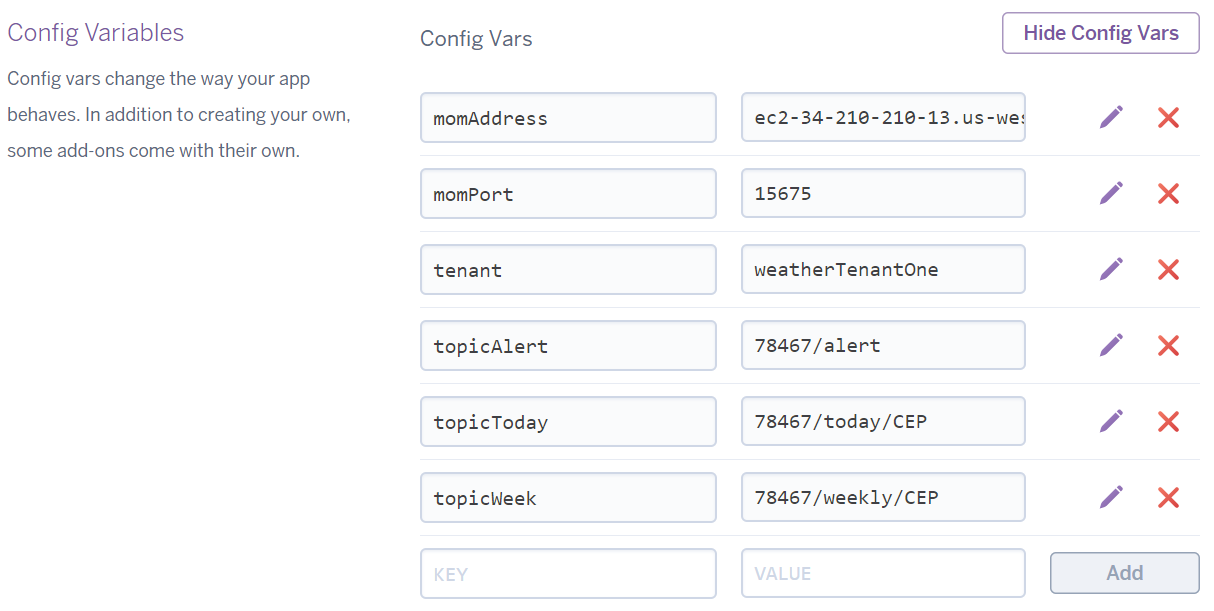
\includegraphics[width=1.0\textwidth]{Bilder/Web-herokuEnv.PNG}
	\caption{Konfiguration der Variablen bei Heroku}
	\label{img:herokuConf}
\end{figure} 


\subsection{Jenkins}\label{Jenkins}
TODO

\section{Kostenmodell}
Die anfallenden Kosten sind entlang der verursachenden Leistung und der Skalierungsabhängigkeit unterteilbar. Auf Seite der Leistungen unterscheiden wir zwischen dem Wetterbericht über den Webclient und die App sowie dem MOM-as-a-Service Angebot. Skalierungsseitig gibt es einmalig anfallende Kosten, Fixkosten, die Nutzungsunabhängig anfallen, um den Betrieb sicherzustellen und Variable Kosten die nur entstehen, wenn die in den Fixkosten eingerechneten Instanzen ausgelastet sind und skalieren müssen.

Die RabbitMQ läuft in einem Docker Container bei Amazon Web Services auf einer "t2.micro" Instanz und kostet bei jährlicher Vorauszahlung \$77 pro Jahr (vgl. https://aws.amazon.com/de/ec2/pricing/reserved-instances/pricing/). Ebenfalls auf einer AWS t2.micro Instanz läuft die Datenbank, somit fallen dafür ebenfalls \$77 jährlich an. Der Client zum auslesen der Daten von openweathermap, wie auch das Complex Event Processing, sind bei Pivotal deployed und kosten jeweils \$21,60 im Monat oder \$259,20 im Jahr(vgl. https://aws.amazon.com/de/ec2/pricing/reserved-instances/pricing). 


Für die Verteilung und den Betrieb der App fallen keine separaten Kosten an, hier sind jedoch die einmalig fälligen \$25,00 für einen Google Play Developer Zugang zu berücksichtigen. Der bei Heroku gehostete Webclient kostet \$7,00 pro Monat oder \$84,00 im Jahr (vgl. https://www.heroku.com/pricing). Zur Berechnung der variablen Kosten für den Webclient wurde der im Abschnitt \nameref{Web-Client} vorgestellte Lasttest verwendet. Daraus ergibt sich, dass der Server gut 1000 Anfragen pro Sekunde bearbeiten kann. Hochgerechnet können so 3,6 Millionen Benutzer die Webseite über einen Zeitraum von einer Stunde besuchen, bevor skaliert werden muss. Unter der Annahme, dass die Kunden im Schnitt nicht öfter als ein mal in der Stunde die Webseite aufrufen ergibt sich so ein Preis von \$0,0233 auf 1000 Benutzer. In den folgenden Tabellen sind die entstehenden Kosten in Dollar pro Jahr bzw. pro 1000 Nutzer pro Jahr ab dem 1001-sten Nutzer angegeben.

\begin{table}
\caption{Tabelle MOM-as-a-Service}
\centering
\begin{tabular}{ccc}
	Funktion & Fix & Variabel \\
	MOM & \$77 & \$ ??? \\
\end{tabular}
\end{table}

\begin{table}
\caption{Tabelle Wetterbericht}
\centering
\begin{tabular}{cccc}
	Funktion 	& Fix		& Variabel	& Einmalig \\
	MOM 		& \$77,00	& \$ ??? 	& \\
	Datenbank	& \$77,00	&			& \\
	Wetter-API 	& \$259,20	&	 		& \\
	CEP 		& \$259,20	& 			& \\
	App			&			&			& \$25,00 \\
	Webclient	& \$84,00	& \$0,0233	& \\
\end{tabular}
\end{table}

In Summe ergeben sich so jährliche Fixkosten in Höhe von \$756,40 und einmalige Kosten von \$25,00.

Decken ließen sich diese Kosten beispielsweise über den Verkauf der App, kostenpflichtigen Accounts für den Webclient oder einer Kombination daraus. Hier darf bei der Berechnung nicht vergessen werden, dass Google 30\% Transaktionsgebühren verlangt und anschließend der Umsatz noch zu versteuern ist. Es bleiben demzufolge nach Abzügen noch 56,7\% des Umsatzes um die Kosten zu decken und eine Gewinnmarge zu erzielen. Bei einem Preis in Höhe von \$0,99 wären für eine Kostendeckung 1393 Verkäufe nötig oder 1000 Verkäufe zu einem Preis von \$1,38. Sollen Accounts für den Webclient verkauft werden, fallen neben den Steuern noch Gebühren an Zahlungsdienstleister an. Diese liegen beispielsweise bei Paypal für Mikrozahlungen zwischen 10\% und 12\% plus einer Währungsabhängigen Pauschale: \$0,05 oder \EUR{0,10} (vgl. https://www.paypal.com/de/webapps/mpp/ua/useragreement-full). Mit dem Dollarpreis gerechnet ergeben sich so bei einem Verkaufspreis von \$0,99 1148 benötigte Verkäufe oder 1000 Verkäufe zum Preis von \$1,08.

Neben dem Wetterbericht ist es durch die Multi-tenant-Fähigkeit möglich die Nutzung der MOM als Service anzubieten. Über die REST-Schnittstelle des Management-Plugins lässt sich die Nutzung protokollieren und somit Nutzungsbasiert abrechnen.

\end{document}
